0%\documentclass[ignorenonframetext]{beamer}

\documentclass[a4paper,titlepage]{article}
\usepackage{beamerarticle}
\includeonlylecture{Lecture 1}
%\includeonlyframes{current}

\usepackage[utf8]{inputenc}
\usepackage{pdfpages}
\usepackage{tikz}
\usepackage{graphicx}
\usepackage{tikzorbital}
\usetikzlibrary{intersections}
\usepackage[version=3]{mhchem}
\usepackage{chemformula}
\usepackage{chessboard, skak}
%\usepackage{skak}

\tikzset{
  level/.style   = { ultra thick, blue },
  connect/.style = { dashed, red },
  notice/.style  = { draw, rectangle callout, callout relative pointer={#1} },
  label/.style   = { text width=2cm }
}

\mode<presentation>{
\usepackage[absolute,overlay]{textpos}
\usetheme{AnnArbor}
\AtBeginLecture{\frame{\Large \insertshortlecture \insertlecture}}
\logo{\includegraphics[height=1cm]{../../graphics/crac}}
}
\setbeamertemplate{headline}{%
    \begin{beamercolorbox}[wd=\paperwidth,ht=2.25ex,dp=1ex,right, rightskip=1mm, leftskip=1mm]{titlelike}
        \inserttitle\hfill\insertauthor\hfill\insertframenumber%
    \end{beamercolorbox}
}

\mode<article>{
\usepackage{textpos}
\usepackage[a4paper, top=1.5in]{geometry}
}
\usepackage{fancyhdr}
\mode<article>{
\pagestyle{fancy}
\fancyhf{}
\lhead{CM3016}
\chead{\footnotesize ELECTRONIC SPECTROSCOPY OF MOLECULES AND ATOMS}
\rhead{S1 2021--2022}
\cfoot{\tiny{version 2021.01}}
\rfoot{\thepage}}

\title{CM3016 -- Physical Chemistry I}
\subtitle{Electronic Spectroscopy}
\author{Stig Hellebust}
\institute{School of Chemistry \\ UCC}
\date{Semester 1 2021/2022}

\newenvironment{titleplainbox}[1]
    {\begin{center}
    #1\\[1ex]
    \begin{tabular}{|p{0.9\textwidth}|}
    \hline\\
    }
    { 
    \\\\\hline
    \end{tabular} 
    \end{center}
    }
\newenvironment{plainbox}
    {\begin{center}
    \begin{tabular}{|p{0.9\textwidth}|}
    \hline\\
    }
    { 
    \\\\\hline
    \end{tabular} 
    \end{center}
    }
    


\begin{document}
\mode<article>{\maketitle}

\begin{frame}
	\titlepage
\end{frame}

\begin{frame}[plain,allowframebreaks=0.75]
 	\tableofcontents
 	\frametitle{Outline}
\end{frame}

%\begin{tikzpicture}
%\drawLevel[elec = up, pos = {(0,0)}, width = 2]{1sH}
%\drawLevel[elec = updown, pos = {(6,-2)}, width = 2]{1sHe}
%
%\drawLevel[elec = pair, pos = {(3,-3)}, width = 2]{sigma}
%\drawLevel[elec = up, pos = {(3,3)}, width = 2]{sigmastar}
%
%\draw[dashed] (right 1sH) -- (left sigma) 
%(right 1sH) -- (left sigmastar) 
%(left 1sHe) -- (right sigmastar) 
%(left 1sHe) -- (right sigma) ;
%
%\node[left] at (left 1sH) {\ce{1s_H}} ;
%\node[right] at (right 1sHe) {\ce{1s_{He}}} ;
%\node[left] at (left sigma) {\(\sigma\)};
%\node[left] at (left sigmastar) {\(\sigma^*\)};
%\end{tikzpicture}

\section*{Scope of this document}
This document contains \emph{all} the material relevant to the aerosol chemistry section of the CM3016 Continuous Assessment and Exam, \emph{including} directed study material. What that means is that everything that is covered in the lectures is contained in this document, and any additional material that is not covered by lectures but included here, makes up the directed study part. 

In other words, this is the only document that is mandatory reading. While this document tells you everything you need to \textit{know} it doesn't necessarily include everything you need to study in order to \textit{understand} the material covered, so the optional reading material provided separately is recommended to assist your understanding of the material.

\lecture[Lecture 1]{Intro and principles}{Lecture 1}

\begin{frame}[<+->]
\frametitle{Electronic Spectroscopy}
\begin{itemize}
\item The study of electronic transitions in:
\begin{itemize}
\item Atoms, or
\item Molecules
\end{itemize}
\item Transitions are associated with:
\begin{itemize}
\item Absorption, or
\item Emission
\end{itemize}
\item Atoms have only electronic degrees of freedom
\item Molecules also have vibrational and rotational degrees of freedom
\item Consequently, electronic spectra of atoms are much simpler than those of molecules
\item Electronic transitions depend on \emph{electronic structure}
\item[\(\implies\)] this means we have to understand \emph{quantum numbers}
\end{itemize}
\end{frame}

\begin{frame}
\frametitle{Analytical Techniques}

Atomic Spectra
\begin{itemize}
\item Atomic Emission, AES
\item Atomic Absorption, AAS
\item Auger Electron Spectroscopy
\item X-Ray Electron Spectroscopy
\end{itemize}
Polyatomic molecules
\begin{itemize}
\item UV-Vis absorption
\item Fluorescence
\item Phosphorescence
\item UV Photoelectron Spectroscopy
\end{itemize}
\end{frame}

\section{Electronic structure, quantum numbers and energies}
\subsection{Quantum numbers}
\label{quantno}

\begin{frame}
\frametitle{Quantum numbers revisited}

There are four quantum numbers. We'll get back to them later, but for now let us accept that they describe the electronic structure of atoms and molecules, i.e. size and shape of the electronic orbitals. They are:

\begin{description}
\item[n :] This is the main energy level, or \textit{electron shell}. Higher numbers indicate higher energy levels and increasing distance form the nucleus. \(n \in [1,\rightarrow\rangle\)
\item[\(\ell\) :] This is the angular quantum number and it describes the shape of the electronic orbital. Also called \textit{subshell}. \(\ell \in [0,n-1]\). 
\item[\(m_\ell\) :] This is the magnetic quantum number. It describes the \textit{orientation} of the electronic orbital. \(m_\ell \in [-l,+l]\)
\item[\(m_s\) :] This is the electron \textit{spin}. \(s\in [-\frac{1}{2},\frac{1}{2}]\)
\end{description}
\end{frame}

\subsubsection{Shells, orbitals, configurations and states}
\begin{frame}
\frametitle{Shells, Subshells, orbitals and electron configurations}

\medskip So there are multiple possible values and each unique combination can only describe one electron in an atom, i.e. no two electrons can have the same set of four numbers in the same atom.\newline
\vspace{1cm} \mode<presentation>{\tiny}
\begin{tabular}{lp{1cm}p{1.2cm}p{1.9in}|p{1.2cm}p{1.5cm}p{2cm}}
\textit{n} & \textit{orbitals} & name of orbital & orientations & \# \newline orbitals \newline (\(n^2\)) & \# electrons in orbitals (2(2\(\ell\) + 1) )& \# electrons in shell (\(2n^2\))\\\hline
1 & \(\ell=0\)  & s & \(m_\ell=0\) & 1 & 2 & 2\pause\\\hline
2 & \(\ell=0\) \newline \(\ell = 1\) & s \newline p & \(m_\ell=0\) \newline \(m_\ell = -1,0,+1\) & 1\newline 3 & 2 \newline 6 & 8\pause\\\hline
3 & \(\ell = 0\) \newline \(\ell=1\) \newline \(\ell=2\) & s\newline p\newline d & \(m_\ell=0\) \newline \(m_\ell = -1,0,+1\) \newline \(m_\ell=-2,-1,0,+1,+2\) & 1\newline 3\newline 5 & 2 \newline 6 \newline 10 & 18\pause\\\hline
4 & \(\ell=0\) \newline \(\ell=1\) \newline \(\ell=2\) \newline \(\ell=3\) & s\newline p \newline d\newline f & \(m_\ell=0\) \newline \(m_\ell = -1,0,+1\) \newline \(m_\ell=-2,-1,0,+1,+2\) \newline \(m_\ell = -3,-2,-1,0,+1,+2,+3\) & 1\newline 3\newline 5\newline 7 & 2\newline 6\newline 10\newline 14 & 32 \\\hline
\end{tabular}
\end{frame}

\begin{frame}
So each orbital is described by three numbers, \(n,\ \ell\) and \(m_\ell\).
\bigskip
Each electron is uniquely described by the four quantum numbers, including spin. For example, an electron described by the numbers \{n=3,\(\ell\)=1,\(m_\ell\)=-1,\(m_s = +\frac{1}{2}\)\} is an electron in the 3rd shell's \(p_x\)-orbital with spin up. Note that each orbital can accommodate 2 electrons if they have paired spin (\textit{paired} meaning \textit{opposite} spin, i.e. \(m_{s_1} \ne m_{s_2}\))\par
\bigskip
Each orbital characterised by particular values of n and \(\ell\) can accommodate 2(2\(\ell\) + 1) electrons, because \(m_\ell\) can take 2\(\ell\)+1 values and \(m_s\) can take 2.
\end{frame}

\begin{frame}
\frametitle{Orbitals in \textit{s, p and d subshells}}
\begin{figure}[h!]
\centering
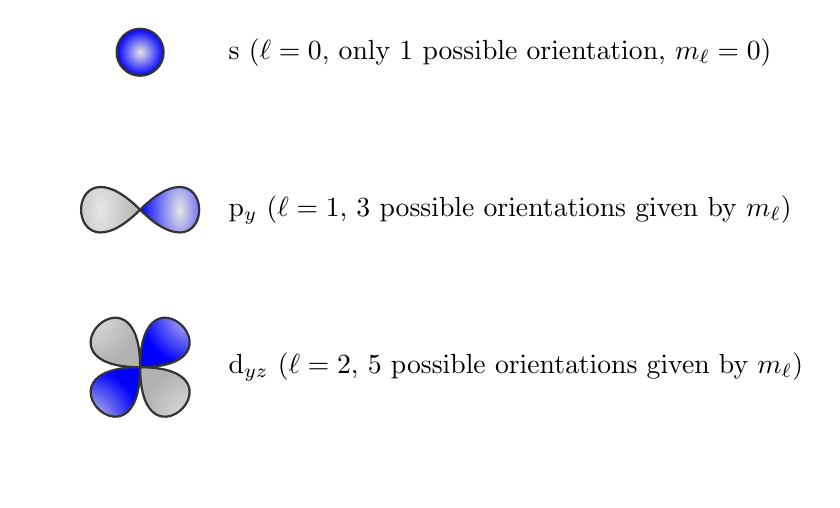
\begin{tikzpicture}
\orbital[pos = {(0,5)}]{s}
\node[right] at (1,5) {s (\(\ell=0\), only 1 possible orientation, \(m_\ell=0\))};

\orbital[pos = {(0,3)}]{py}
\node[right] at (1,3) {p$_y$ (\(\ell=1\), 3 possible orientations given by \(m_\ell\))};
%\orbital[pos = {(4,5)}]{py}
%\node[above] at (4,6) {p$_y$};
%\orbital[pos = {(6,5)}]{pz}
%\node[above] at (6,6) {p$_z$};

%\orbital[pos = {(0,2)}]{dxy}
%\node[above] at (0,3) {d$_{xy}$};
%\orbital[pos = {(2,2)}]{dxz}
%\node[above] at (2,3) {d$_{xz}$};
\orbital[pos = {(0,1)}]{dyz}
\node[right] at (1,1) {d$_{yz}$ (\(\ell = 2\), 5 possible orientations given by \(m_\ell\))};

%\orbital[pos = {(0,-5)}]{dx2y2}
%\node[below] at (0,-6) {d$_{x^2-y^2}$};
%\orbital[pos = {(4,1)}]{dz2}
%\node[right] at (5,1) {d$_{z^2}$};
\end{tikzpicture}
\caption{s orbitals are spherically shaped, while p and d orbitals have lobes.}
\end{figure}
\end{frame}

\begin{frame}
\frametitle{Shells, Subshells, Orbitals, Configurations and States}
\begin{description}
\item[Shell:] all orbitals having same value of n\newline
n = 1,2,3,4 \(\rightarrow\) Shells K,L,M,N
\item[Subshell:] a set of values of n and \(\ell\) 
\item[Orbital:] Regions with different values of \(m_\ell\) within a subshell
\item[Configuration:] The way in which electrons are distributed among various orbitals. \textbf{This can give rise to more than one \textit{State}}
\item[State] The wavefunction describes a \textbf{state}
\end{description}
\end{frame}

\subsection{Energies}
\subsubsection{The quantum mechanical form of the energy}
\label{poly}
The energy can be described by the Hamiltonian in polar coordinates. The Hamiltonian is just an operator which considers the kinetic energies and the potential energies of a system. It was first used as a reformulation of Newtonian mechanics, but it is now very important in quantum mechanics. The Hamiltonian describes the energy of a system.

\begin{frame}
\frametitle{Energy of single electron systems}
\only<1>{
\medskip For a \underline{Hydrogen atom:}
\[ H=-\frac{\hbar^2}{2\mu}\bigtriangledown^2 - \frac{Ze^2}{4\pi\varepsilon_0r}\]
where \(\hbar = \frac{h}{2\pi}\)\newline\medskip \(\mu = \) reduced mass \(=\frac{m_em_p}{m_e+m_p}\). \(m_e\) is the electron mass and \(m_p\) is the mass of the proton.\newline


\bigskip the second term is the Coulombic potential energy for attraction between charges of a single electron and nucleus of charge Z at distance r. We can call this term \textit{V}.\newline
}
\only<2>{
\medskip The first term is the kinetic energy term, \(-\frac{\hbar^2}{2\mu}\bigtriangledown^2\), which we can call \textit{T}. It is given by the \textit{Laplacian}, \(\bigtriangledown^2\):\newline

\[ \bigtriangledown^2 = \frac{1}{r^2sin\Theta}\left[sin\Theta\frac{\delta}{\delta r}\left(r^2\frac{\delta}{\delta r}\right) + \frac{\delta}{\delta\Theta}\left(sin\Theta\frac{\delta}{\delta\Theta}\right) + \frac{1}{sin\Phi}\frac{\delta^2}{\delta\Phi^2}\right]\]

\bigskip where r = distance of point P from origin\newline
\(\Theta\): co-latitude\newline
\(\Phi\): azimuth\newline

\medskip \textbf{The potential and kinetic energy terms are
added together to form the Hamiltonian, H = T + V}
}
\end{frame}

\subsection{The hydrogen atom}

% Hndwritten notes H1-H3 here in frame
The hydrogen atom (as well as hydrogen-like atoms which have only one electron) is
unique in that it has only a single electron – this means that there are no interactions
between multiple electrons in the system. This greatly simplifies solving the Schrödinger
equation, which can be solved analytically in the case of the hydrogen atom, but must be
analysed using numerical methods in the case of multi-electron atoms. Despite these
differences between hydrogen and other atoms, the hydrogen atom provides a useful
starting point for describing the energies and spatial distribution of electrons in orbitals,
as well as the introducing the quantum numbers needed to study the describe the state of
the atom. We will see that much of the focus in describing the state of atoms depends on
careful consideration of the angular momentum of the electrons. Once the atom is
accurately described, we can then consider the selection rules governing transitions
between different states in a given atom.

The hydrogen atom has a single electron and a nucleus. The quantum mechanical model
of the system needs to describe the kinetic and potential energies in the system. For a
single electron interacting with a nucleus of charge Z, the potential energy is described by
the Coulombic potential.


The solutions to the Schrödinger equation (see section \ref{schrod}) give us both the possible energies of the
system, as well as the possible wavefunctions. As with other quantum mechanical
problems, we find that quantum numbers arise that are needed to describe various aspects
of the solution.\newline

\medskip The possible energies of the Hydrogen atom are:
\[E_n = -\frac{Z^2\mu e^4}{32\pi^2\varepsilon^2_0\hbar^2n^2}\]
\medskip where n is the \textit{principal quantum number}, n = 1, 2, 3, ...
The other quantum numbers that are required to describe the electron \textit{orbitals} are the orbital angular momentum quantum number, \(\ell\), (also termed the azimuthal quantum number) and the magnetic quantum number, \(m_l\). We talked about these in section \ref{quantno} where their possible values are given.

These numbers describe the \textit{orbital}, but to describe the electron fully we also need the \textit{electron spin quantum number}, \(m_s\)

\subsection{Atoms with multiple electrons}

The hydrogen atom provides us with a useful initial
model of atomic energy levels, orbital shapes, and the
quantum numbers needed to describe the system. For
multi-electronic atoms, solving the Schrödinger
equation becomes much more complex because we now
need to account not only for Coulombic interactions
between the nucleus and more electrons, but we also
must account for electron-electron repulsion. In this
case, exact solutions are no longer possible. As a first
result, we find that the interactions between electrons
lifts the degeneracy of the hydrogenic energy levels.
Thus, 2s and 2p orbitals no longer have the same
energy as they do in the hygrogen atom. In this case,
we find that the s orbitals are lower in energy than the p
orbitals. This effect arises because s electrons are closer to the nucleus than p electrons,
and the influence of electron-electron repulsion is relatively small compared to the
electron-nucleus interaction.

The order in which electrons fill available orbitals within
an atom is determined by the Aufbau principle (German:
“building up”), in which electrons are placed in the
lowest available energy level.

In filling the orbitals, we also need to take into account
the Pauli exclusion principle, which we can state as: \begin{quotation}
No two electrons can have the same four quantum
numbers (n, \(\ell\), \(m_\ell\), \(m_s\)) \end{quotation}
Another expression of the Pauli exclusion principle is
that there can be a maximum of two electrons per orbital
and that their spins must be antiparallel.

Once we have obtained the correct electron configuration by placing all available
electrons in the correct orbitals, we are now in a position to describe the state of the atom.
Doing so is requires careful consideration of the angular momentum of
the system.

\bigskip For a \underline{Polyelectronic atom}:\newline
\[ H=-\frac{\hbar^2}{2m_e}\sum_i\bigtriangledown^2 - \sum_i\frac{Ze^2}{4\pi\varepsilon_ir} + \sum_{i<j}\frac{e^2}{4\pi\varepsilon_0r_{ij}}\]

\medskip This equation contains summations over all electrons, i, and there is now a \textit{third} term. The new terms due to Coulombic \textit{repulsion} between pairs of electrons at distance \(r_{ij}\)

\begin{frame}
\frametitle{Energy of polyelectronic atoms}
\only<1>{\bigskip Consider an atom that contains a nucleus of mass \(m_n\) with a positive charge of \textit{+Ze} and \textit{N} electrons. 

\medskip This means we have N+1 particles that can all have kinetic energy. The quantum mechanical Hamiltonian will therefore have \textbf{N+1 kinetic energy terms} of the form \(-\hbar/(2m)\bigtriangledown^2\). Each of the electrons will be attracted to the positively charged nucleus. 
\medskip The \textbf{attractive coulombic interactions} will lead to \textbf{N terms} in the potential of the general form \(-Ze^2/r_i\), where \(r_i\) is the distance of electron \textit{i} from the nucleus. We use electrostatic units to avoid having to put the factor \(4\pi\varepsilon_0\) in the denominator. 
}
\only<2>{
\medskip Each pair of electrons with the same charge will experience a \textbf{repulsive interaction} that produces a potential term of the form \(e^2/r_{ij}\), where \(r_{ij}\) is the distance between electrons \textit{i} and \textit{j}. 

\medskip The number of such pairwise interactions is the number of combinations of N objects two at a time: \(C(N,2) = \frac{N!}{(N-2)!(2)!} = \frac{N(N-1)}{2}\). 


\medskip For the Lithium atom, with three electrons, there are 3(2)/2 = 3 repulsion terms. \textbf{For Sodium, with 11 electrons, there are 11(10)/2 = 55 terms}. 

\medskip The Hamiltonian for the sodium atom will therefore contain 12 kinetic energy terms, 11 nuclear-electron attraction terms and 55 electron-electron repulsion terms.
}
\end{frame}

\begin{frame}
\frametitle{Born-Oppenheimer approximation}
\only<1>{
For polyelectric atoms the equation can only be solved by approximation. 

\smallskip One such approximation is called the \textbf{\textit{Born-Oppenheimer}} approximation. 

\smallskip This notes that the mass of the nucleus in the nuclear-electron attraction term is much larger than the electron mass. 

\smallskip The large mass means that the nucleus is movinig very slowly compared to the lighter electrons. 

\smallskip We therefore assume that we can remove the kinetic energy terms for the nuclei from the Hamiltonian. We can separate the problems of nuclear and electronic motions.
}

\only<2>{
\medskip \textbf{\textit{The Hartree approximation}} assumes that the electrons are independent, and interact only via the mean-field Coulomb potential. 

This yields one-electron Schrödinger equations:

\[H \approx -\frac{\hbar^2}{2m_e}\sum_i\bigtriangledown^2 - \sum_i\frac{Ze^2}{4\pi\varepsilon_ir} + \sum_iV(r_i)\]
}

\only<3>{
\medskip We're not going to worry about the Hamiltonian any more. 

\smallskip But we can note that 
The ORBITAL energies, \(E_i\) vary with the principal quantum number n, but also with orbital angular momentum quantum number \(\ell\) (=0,1,2,...).
}
\end{frame}

%Orbital energies vary with the principal quantum number, n, but also with orbital angular momentum quantum number \(\ell\).

\subsubsection{The Schrödinger equation}
\label{schrod}

\begin{frame}
\frametitle{Schrödinger's wave function}
\only<1>{
The potential and kinetic energy terms are
added together to form the Hamiltonian, H = T + V, and inserted in the time-independent
Schrödinger equation:

\begin{align*}
-\hbar^2\frac{\delta^2\Psi}{\delta x^2} &= p^2\Psi\\
\hat{H}\Psi &= E\Psi
\end{align*}

where:\newline \(\Psi\) is the wavefunction\newline H is the Hamiltonian operator and \newline E is the energy.
}
\end{frame}
We will not talk of the Schrödinger equation again. All we need to know is that the Schrödinger wave function defines the behaviour of the electron in three dimensions, and that the possible wavefunction solutions to the Schrödinger equation define the orbital shapes, e.g. like those in figure \ref{orbshapes}

\begin{frame}
\frametitle{Orbital shapes}
The solutions to the wavefunction define the orbitals
\begin{figure}[h!]
\centering
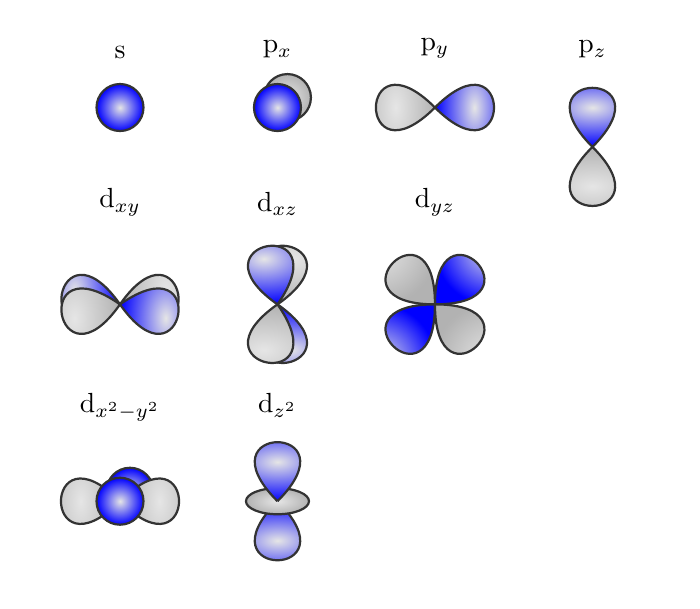
\begin{tikzpicture}
\orbital[pos = {(0,5.5)}]{s}
\node[above] at (0,6) {s};
\orbital[pos = {(2,5.5)}]{px}
\node[above] at (2,6) {p$_x$};
\orbital[pos = {(4,5.5)}]{py}
\node[above] at (4,6) {p$_y$};
\orbital[pos = {(6,5)}]{pz}
\node[above] at (6,6) {p$_z$};

\orbital[pos = {(0,3)}]{dxy}
\node[above] at (0,4) {d$_{xy}$};
\orbital[pos = {(2,3)}]{dxz}
\node[above] at (2,4) {d$_{xz}$};
\orbital[pos = {(4,3)}]{dyz}
\node[above] at (4,4) {d$_{yz}$};

\orbital[pos = {(0,0.5)}]{dx2y2}
\node[below] at (0,2) {d$_{x^2-y^2}$};
\orbital[pos = {(2,0.5)}]{dz2}
\node[below] at (2,2) {d$_{z^2}$};
\end{tikzpicture}
\caption{s orbitals are spherically shaped, while p and d orbitals have lobes. 
Different p and d orbitals with the same principle quantum number have different
orientations in space. As the principle quantum number increases, so the distance from
the nucleus also increases.}\label{orbshapes}
\end{figure}
\end{frame}

\begin{frame}
\frametitle{The significance of quantum numbers}
So this reminds us of the \underline{physical significance of the quantum numbers:}
\begin{enumerate}
\item The principle quantum number, n, indicates the energy of the orbital and its
distance from the nucleus. Smaller values of n mean that the electron is closer
to the nucleus.
\item The orbital angular momentum quantum number, \(\ell\), indicates the shape of the
orbital. Moreover, it also indicates the magnitude of the angular momentum
of the electron in the orbital and the associated magnetic moment of the
orbital.
\item The magnetic quantum number, \(m_\ell\), indicates the orientation in space of the
orbital. Specifically, it indicates the direction of the angular momentum and of
the associated magnetic moment of the orbital.
\end{enumerate}
\end{frame}

\lecture[Lecture 2]{Transitions, the Franck-Condon principle and energies}{Lecture 2}

\subsubsection{Electronic Transitions}
\medskip

\begin{frame}
\frametitle{Electronic energy levels and electron configurations}
\begin{columns}[onlytextwidth]
\begin{column}{.45\textwidth}

\visible<1->{
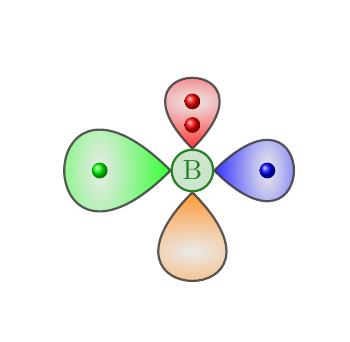
\begin{tikzpicture}
\satom[name=B, color=green!50!black]{
	red/90/north/2/.8,
	blue/0/east/1/.9,
	orange/270/south/0/1,
	green/180/west/1/1.2}
\end{tikzpicture}
}
\end{column}

\begin{column}{.45\textwidth}
\visible<2>{
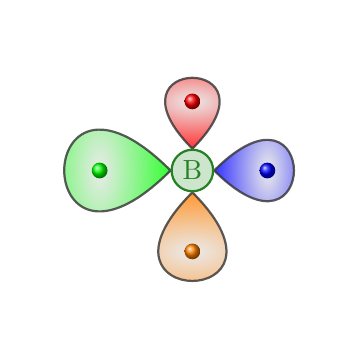
\begin{tikzpicture}
\satom[name=B, color=green!50!black]{
	red/90/north/1/.8,
	blue/0/east/1/.9,
	orange/270/south/1/1,
	green/180/west/1/1.2}
\end{tikzpicture}
}

\end{column}
\end{columns}
\visible<2>{Energy levels are related to where the electrons are in the molecule}
\end{frame}

\begin{frame}[label=current]
\frametitle{The energy level diagrams}
\only<1>{
The Molecular orbital diagram -- example: formaldehyde

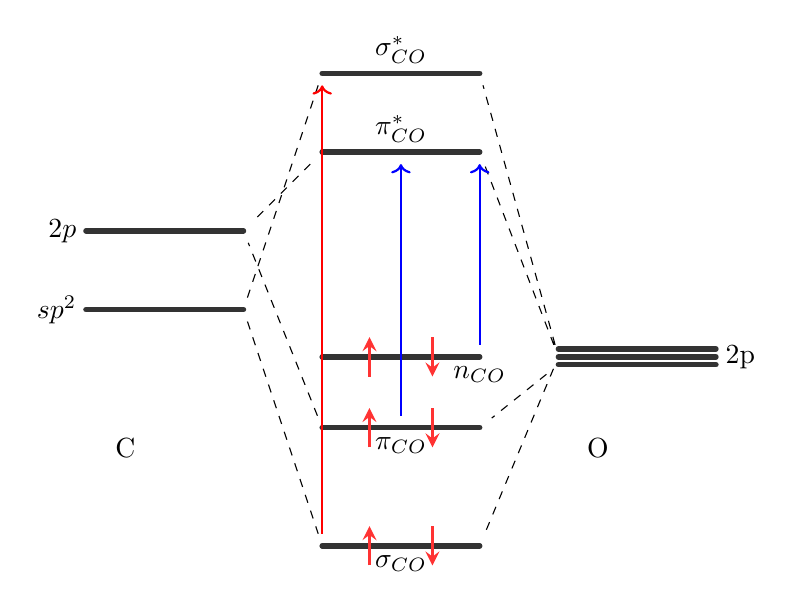
\begin{tikzpicture}
\drawLevel[elec = no, pos = {(0,0)}, width = 2]{sp2}
\drawLevel[elec=no,pos={(0,1)},width=2]{2p}
\drawLevel[elec = no, pos = {(6,-0.5)}, width = 2]{o2px}
\drawLevel[elec = no, pos = {(6,-0.6)}, width = 2]{o2py}
\drawLevel[elec = no, pos = {(6,-0.7)}, width = 2]{o2pz}

\drawLevel[elec = pair, pos = {(3,-3)}, width = 2,spinlength=0.5]{sigma}
\drawLevel[elec = pair, pos = {(3,-1.5)}, width = 2,spinlength=0.5]{pi}
\drawLevel[elec = pair, pos = {(3,-0.6)}, width = 2,spinlength=0.5]{n}
\drawLevel[elec = no, pos = {(3,3)}, width = 2,spinlength=0.5]{sigmastar}
\drawLevel[elec = no, pos = {(3,2)}, width = 2,spinlength=0.5]{pistar}

\draw[dashed] (right sp2) -- (left sigma)
 (right sp2) -- (left sigmastar)
 (left o2py) -- (right sigmastar)
 (left o2py) -- (right sigma) 
 (left pi) -- (right 2p)
 (left o2pz) -- (right pi)
 (left o2py) -- (right pistar)
 (left pistar) -- (right 2p)
 ;
 \draw[->, red,thick] (left sigma) -- (left sigmastar);
 \draw[->, blue,thick] (middle pi) -- (middle pistar);
 \draw[->, blue,thick] (right n) -- (right pistar) ;

\node[left] at (left sp2) {\(sp^2\)} ;
\node[left] at (left 2p) {\(2p\)} ;
\node[right] at (right o2py) {2p} ;
\node[below] at (middle sigma) {\(\sigma_{CO}\)};
\node[below] at (middle pi) {\(\pi_{CO}\)};
\node[below] at (right n) {\(n_{CO}\)};
\node[above] at (middle sigmastar) {\(\sigma_{CO}^*\)};
\node[above] at (middle pistar) {\(\pi_{CO}^*\)};
\node[above] at (0.5,-2){C};
\node[above] at (6.5,-2){O};
\end{tikzpicture}
}

\only<2>{
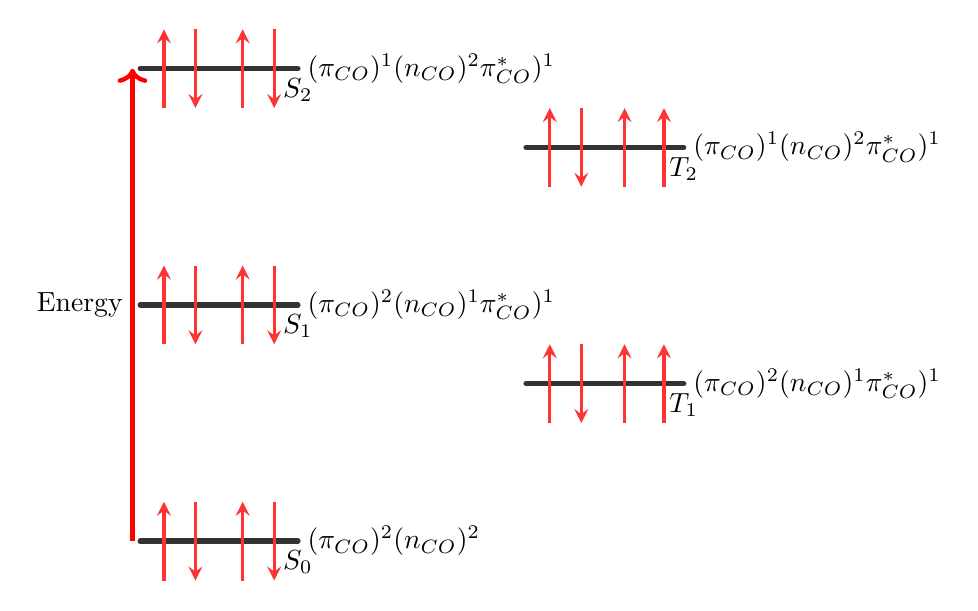
\begin{tikzpicture}
\drawLevel[elec=updown,pos={(0.1,-3)},width=1]{S0}
\drawLevel[elec=updown,pos={(1.1,-3)},width=1]{S00}
\node[right] at (right S00){\((\pi_{CO})^2(n_{CO})^2\)};
\node[below] at (right S00){\(S_0\)};
\draw[->,ultra thick,red] (0,-3) -- (0,3);
\node[left] at (0,0){Energy};

\drawLevel[elec=updown,pos={(0.1,0)},width=1]{S1}
\drawLevel[elec=updown,pos={(1.1,0)},width=1]{S11}
\node[right] at (right S11){\((\pi_{CO})^2(n_{CO})^1\pi^*_{CO})^1\)};
\node[below] at (right S11){\(S_1\)};

\drawLevel[elec=updown,pos={(0.1,3)},width=1]{S2}
\drawLevel[elec=updown,pos={(1.1,3)},width=1]{S22}
\node[right] at (right S22){\((\pi_{CO})^1(n_{CO})^2\pi^*_{CO})^1\)};
\node[below] at (right S22){\(S_2\)};

\drawLevel[elec=updown,pos={(5,-1)},width=1]{T1}
\drawLevel[elec=up,pos={(6,-1)},width=.5]{T11}
\drawLevel[elec=up,pos={(6.5,-1)},width=.5]{T12}
\node[right] at (right T12){\((\pi_{CO})^2(n_{CO})^1\pi^*_{CO})^1\)};
\node[below] at (right T12){\(T_1\)};

\drawLevel[elec=updown,pos={(5,2)},width=1]{T2}
\drawLevel[elec=up,pos={(6,2)},width=.5]{T22}
\drawLevel[elec=up,pos={(6.5,2)},width=.5]{T23}
\node[right] at (right T23){\((\pi_{CO})^1(n_{CO})^2\pi^*_{CO})^1\)};
\node[below] at (right T23){\(T_2\)};

\end{tikzpicture}
}

\only<3>{
The 2D Jablonski diagram -- energy and internuclear distance

\begin{center}
\includegraphics[width=.9\textwidth]{../../graphics/2Djablonski}
\end{center}
}
\end{frame}

\begin{frame}
\frametitle{\textbf{Spectroscopy} provides information on \textbf{transitions between molecular states}.}
\only<1>{
\par\medskip Electronic spectroscopy of a molecule is linked to its \emph{energy levels}, which are determined by structure and chemical composition \(\implies\) UV-Vis spectroscopy is a useful tool for identifying molecules. 

\par\medskip Bond lengths and chemical reactivity of excited-state species can be quite different from the ground states.

In an electronic transition there is a transition moment, \(R_{nm}\) from the wavefunctions \(\Psi_m\) and \(\Psi_n\) of the combining states.\newline

\medskip For interactions with the electric component of the radiations, \(\mu\) = electric dipole moment \(= \sum_iq_ir_i\)\newline
}
\only<2>{
\medskip VIBRONIC TRANSITIONS: Vibrational transition accompanying an electronic transition. The vibronic transtion moment, \(R_{ev}\):
\[ R_{ev} = \int\Psi^{`*}_{ev}\mu\Psi^{``}_{ev}d\tau_{ev}\]

\medskip \(\Psi^{'}\) and \(\Psi^{``}\) are the vibronic wave functions of the upper (\(\Psi^{'}\)) and lower (\(\Psi^{``}\)) states. \newline

\medskip Remember the Born-Oppenheimer approximation (Section \ref{poly}). This assumes that \(\Psi_{ev} = \Psi_e\Psi_v\).\newline
}
\only<3>{
\medskip This is useful because we can write:

\[R_{ev} = \int\int\Psi^{`*}_e\Psi^{`*}_v\mu\Psi^{``}_e\Psi^{``}_vd\tau_{ev}dr\]

\medskip If we integrate this with respect to electron coordinates \(\tau_e\) we get:

\[R_{ev} = \int\Psi^{`*}_vR_e\Psi^{``}_vdr\]

\medskip where r is the internuclear distance and \(R_e\) is the electronic transition moment, \(R_e = \int\Psi^{`*}_e\mu\Psi^{``}_ed\tau_e\)
}
\only<4>{
\medskip This is useful because the Born-Oppenheimer approximation lets us assume that the nuclei can be regarded as stationary. In the equation this means that \(R_e\) can be moved outside the integral (because it is independent of r)

\[R_{ev} = R_e\int\Psi^{`*}_v\Psi^{``}_vdr\]

\medskip The integral in this equation is the \textit{Vibrational overlap integral}\newline
\medskip The overlap is a measure of how much the two vibrational wave functions overlap. The square of the integral is the \textbf{Frank-Condon factor}.
}
\end{frame}

\subsection{Frank-Condon principle}

\begin{frame}[shrink]
\frametitle{The Franck Condon Principle}
\begin{columns}[onlytextwidth]
\begin{column}{.3\linewidth}
\begin{figure}[h!]
\includegraphics[width=6\TPHorizModule]{../../graphics/FC1}
\caption{\footnotesize Franck-Condon principle energy diagram. The potential wells are shown favouring transitions between \(\nu = 0\) and \(\nu = 2\)}
\end{figure}
\end{column}
\begin{column}{.6\linewidth}
\fbox{\parbox{\linewidth}{\small The \emph{Frank Condon Principle} states that during an electronic transition, a change from one vibrational energy level to another will be more likely to happen if the \emph{\underline{two vibrational wave functions overlap}} more significantly }}
\begin{figure}[h!]
\includegraphics[width=6\TPHorizModule]{../../graphics/FC2}
\end{figure}
\end{column}
\end{columns}
\end{frame}


\begin{frame}
\frametitle{The Franck-Condon Principle}
\only<1>{
The timescale of an electronic transition is extremely short: \(<10^{-15}\) s  (that is, subfemtosecond). Compare this to the time scale of nuclear motion during bond vibtrations:\newline
\textcolor{red}{{e.g 1000 \(cm^{-1} \rightarrow \nu \approx 3\times 10^{13} s^{-1} \rightarrow \Delta t \approx 10^{-14}s\)}} \newline\smallskip
\textbf{The Franck-Condon Principle:}\newline
\begin{quotation}
An electronic transition is so fast compared to nuclear motion that the nuclei still have the same position and momentum immediately after the transition as before it.
\end{quotation}
\medskip
Electronic transitions occur most favourably when the nuclear structure of the initial and final states is similar\newline
\medskip
%In a configurational coordinate diagram, electronic transitions are represented by \underline{vertical lines}
}

\only<2>{
As with the Born-Oppenheimer approximation, this difference between the velocities of
the electrons and the nuclei is taken into account by the Frank-Condon Principle, which
relates to transitions between electronic states. 

\medskip This means that electronic transitions are represented by \emph{vertical lines} (implying that the
nuclei positions is unchanged) in a configurational coordinate diagram (the type of
energy level diagrams we have often seen, e.g. figure \ref{jab1}):
}
\end{frame}

%\begin{frame}[allowframebreaks]
%\frametitle{Absorption conditions}
%\fbox{Absorption can occur if: \colorbox{yellow}{\textcolor{black}{\(E_{exc} = E^* - E_0 = h\nu = hc/\lambda\)}}}
%
%\begin{description}
%\item[\(E_{exc}\)] Electronic excitation energy
%\item[\(E^*\)] Energy of the excited state
%\item[\(E_0\)] Energy of the initial state
%\item[h] Planck's constant
%\item[\(\nu\)] Frequency of absorbed radiation
%\item[c] Speed of light
%\item[\(\lambda\)] Wavelength of absorbed radiation
%\end{description}
%
%\begin{itemize}
%\item[ ] \includegraphics[height=2in]{../../graphics/absorption}
%\item Energy of the molecule has increased by the energy of the absorbed photon
%\end{itemize}
%
%\end{frame}

%\begin{frame}
%\frametitle{The Jablonski-State diagram}
%\begin{itemize}
%\item[] \includegraphics[width=\linewidth]{../../graphics/jablonski_1D}
%\item This 1-D representation of the Jablonski diagram shows \textit{\underline{energy differences only}}
%\end{itemize}
%\end{frame}
%
%\begin{frame}
%\frametitle{2-D configuration co-ordinate Jablonski diagram}
%\centering
%\begin{figure}[h!]
%\includegraphics[width=\linewidth]{../../graphics/2Djablonski}
%\caption{This 2-D representation of the Jablonski diagram shows \textit{\underline{energy and geometry changes}}, \textit{i.e.} shape changes due to bonds extending or changing angle}
%\end{figure}
%\end{frame}
%
%\begin{frame}
%\frametitle{2-D Jablonski diagram}
%\begin{figure}[h!]
%\includegraphics[width=\linewidth]{../../graphics/2Djablonski2}
%\caption{\fcolorbox{black}{yellow}{\textcolor{black}{\parbox{\textwidth}{Note that IC and ISC occur with no change in energy!}}}}
%\end{figure}
%\end{frame}


\begin{frame}[<+->]
\frametitle{The Franck Condon Principle}
\begin{itemize}
\item Since electronic transitions are \textit{\underline{very fast compared with nuclear motions}}, vibrational levels are favoured when they correspond to a minimal change in the nuclear coordinates
\item In other words, because electronic transitions are essentially instantaneous (\(\approx10^{-15}\) seconds) there is little or no geometry change in the molecular system
\item As a result, \textit{\underline{optical transitions}} on the 2-D Jablonski diagram are \newline \textit{\underline{represented by lines of length h\(\nu\)}} \textemdash nuclei do not move in the interim
\end{itemize}
\end{frame}

% Handwritten notes H4-H5 here in frame
\subsection{Absorption band shapes}
\label{bandshapes}
\begin{frame}
\frametitle{Spectroscopy and transition energies}
\only<1>{
Electronic Spectroscopy of a molecule is linked to its energy levels, which are determined by structure and chemical composition

 \(\implies\) UV-Vis Spectroscopy is a useful tool for identifying molecules. 
 
 \medskip Bond lengths and chemical reactivity of excited-state species can be quite different from the ground state.
}

\only<2>{
\frametitle{Transition energies}
\begin{description}
\item[Rotational and Vibrational transitions:] of the order of 1 and 10 kJ mol\(^{-1}\), respectively
\item[Photon energies associated with electronic transitions:] of the order of 200 to 1000 kJ mol\(^{-1}\)
\end{description}

The absorption bands that we see in a spectrum can give us a clue to the changes in nuclear coordinates during an electronic transition
}
\end{frame}


%\begin{figure}[h!]
\begin{frame}
\frametitle{Absorption bands with no change in radius, \(r''_e \approx r'_e\)}
\begin{columns}[onlytextwidth]
\begin{column}{.5\textwidth}
\includegraphics[width=6\TPHorizModule]{../../graphics/bandshapes1}
\end{column}

\begin{column}{.4\textwidth}
If the nuclear coordinates are approximately equal, i.e. \(r''_e \approx r'_e\) in the ground and electronic states, then the strongest absorption is the 0-0 transition
\end{column}
\end{columns}
\end{frame}

%\end{figure}

%\begin{figure}[h!]
\begin{frame}
\frametitle{Absorption bands for transitions causing \(r''_e < r'_e\)}
\begin{columns}[onlytextwidth]
\begin{column}{.5\textwidth}
\includegraphics[width=6\TPHorizModule]{../../graphics/bandshapes2}
\end{column}

\begin{column}{.4\textwidth}
If the atomic radious is smaller in the excited state than in the ground state, \(r''_e < r'_e\), then the absorption spectrum could look a bit symmetric, like this
\end{column}
\end{columns}
\end{frame}

%\end{figure}

%\begin{figure}[h!]
\begin{frame}
\frametitle{Absorption bands for transitions causing greater separation, \(r''_e > r'_e\), leading to dissociation}
\only<1>{
\begin{columns}[onlytextwidth]
\column{.5\textwidth}
\includegraphics[width=6\TPHorizModule]{../../graphics/bandshapes3}
\column{.5\textwidth}
\includegraphics[width=6\TPHorizModule]{../../graphics/2DJablonski4}
\par\(r'_e > r''_e\) is a common situation because electron promotion is from a bonding orbital to a non-bonding orbital or anti-bonding orbital
\end{columns}
}

\only<2>{
\includegraphics[width=\textwidth]{../../graphics/ClO}
}
\end{frame}

The excited state has increased atomic radius \(r''_e > r'_e\) because of weaker bond
%\end{figure}

%\begin{figure}[h!]
\begin{frame}
\frametitle{Excitation to unbound states}
\includegraphics[height=3in]{../../graphics/bandshapes4}
\end{frame}
%\end{figure}

\begin{frame}
\frametitle{Examples}
\only<1>{
\begin{figure}[h]
\begin{center}
\includegraphics[width=6\TPHorizModule]{../../graphics/2Djablonski3}
%\begin{textblock}{6}(6,0)
\caption{In this energy diagram, the most probable transition is the 2-0 transition. That means the transition between level \(v^{``}_0\) in the ground state and level \(v^{'}_2\) in the excited state (blue arrow).
\(r_e^{`} > r_e^{``}\) is oten the case because electron promotion is from a bonding orbital to a non-bonding or anti-bonding orbital.}\label{jab1}
%\end{textblock}
\end{center}
\end{figure}
}
\end{frame}

\begin{frame}
\frametitle{Example: Oxygen}
\begin{center}
\includegraphics[height=3in]{../../graphics/oxygenenergy}
\end{center}
\end{frame}

\begin{frame}
\frametitle{Example: Carbon}
\begin{center}
\includegraphics[height=3in]{../../graphics/carbonenergy}
\end{center}
\end{frame}

\begin{frame}
\frametitle{Example: Hydrogen}
\only<1>{
\begin{center}
\includegraphics[width=3.5in]{../../graphics/hydrogenenergy}
\end{center}
}

\only<2>{
Example potential energy curves for the H\textsubscript{2} molecule. Take note of the following
features of the graph:
\begin{itemize}
\item There are multiple possible excited electronic states of the H\textsubscript{2} molecule.
These correspond to electrons being found in different molecular orbitals
of differing energy.
\item On the right side of the curve, when the nuclei have a large separation, H\textsubscript{2}
dissociates into two H atoms. The difference between the lower and
higher curves is that the lower curves arise from H atoms in the ground
state (1s), whereas for higher energy curves at least one H atom is in a
higher energy state (2s or 2p configurations).
\end{itemize}
}

\only<3>{
\begin{itemize}
\item To form a stable molecule, the curve needs to have a minimum – some
electronic states are purely dissociative and cannot form stable molecules (e.g., 3\(\Sigma^+_u\)).
\item Bound states (those with a potential minimum) give rise to vibrational
levels. Only the ground (v=0) vibrational level is shown on the bound
states below.
\item Transitions between levels are shown as vertical lines (see the Frank-
Condon effect). Note that the only allowed transitions are those that have
the same multiplicity (leftmost superscript).
\end{itemize}
}
\end{frame}



\subsubsection{Dissociation Energies}

%\begin{frame}[shrink]
%\begin{figure}[h!]
%\begin{tikzpicture}[scale=0.65]
%%\draw[step=1cm, gray, very thin] (-5,-5) grid (5,5);
%%ground state
%\draw[thick] (-5,0) .. controls (-2.5,-10)  and (-2,-1) .. (2,-1) .. controls (2,-1) .. (5,-1);
%\path[name path=ground state] (-5,0) .. controls (-2.5,-10)  and (-2,-1) .. (2,-1) .. controls (2,-1) .. (5,-1);
%\path[name path = v0] (-4,-4) -- (-1,-4);
%\path[name intersections={of = ground state and v0}];
%\coordinate (A) at (intersection-1);
%\node[left] at (A) {\(\nu^{``}=0\)};
%\coordinate (B) at (intersection-2);
%\draw (A) -- (B);
%\draw[dashed] (B) -- (5,-4);
%
%%excited state
%\draw[thick] (-5,5) .. controls (-2.5,-5)  and (-2,4) .. (2,4) .. controls (2,4) .. (5,4);
%\path[name path=ex state] (-5,5) .. controls (-2.5,-5)  and (-2,4) .. (2,4) .. controls (2,4) .. (5,4);
%\path[name path = v1] (-4,1) -- (-1,1);
%\path[name intersections={of = ex state and v1}];
%\coordinate (C) at (intersection-1);
%\node[left] at (C) {\(\nu^{`}=0\)};
%\coordinate (D) at (intersection-2);
%\draw (C) -- (D);
%\draw[dashed] (D) -- (2,1);
%
%\draw[<->] (2,4)  -- (2,1); 
%\node[anchor=west] at (2,2.5) {\(D'_0\)};
%\draw[<->]((2,1) -- (2,-4);
%\node[anchor=west] at (2,-2){\(\tilde{\nu_0}\)};
%
%\draw[<->](3,4) -- (3,-4);
%\node[anchor=west] at (3,0){\(\tilde{\nu}_{limit}\)};
%\path[name path = diss] (-5,-0.5) -- (-4,-0.5);
%\path[name intersections={of=ground state and diss}];
%\coordinate (E) at (intersection-1);
%\draw (E) -- (5,-0.5);
%
%\draw[<->](4,4) -- (4,-0.5);
%\node[anchor=west] at (4,2.5){\(\Delta\tilde{\nu}_{atomic} \)};
%\draw[<->](4,-0.5) -- (4,-4);
%\node[anchor=west] at (4,-2){\(D''_0\)};
%
%\node[anchor=south] at (0,-5){\(r\rightarrow\)};
%\end{tikzpicture}
%\caption{
%\(\tilde{\nu}_{limit} = D'_0 + \tilde{\nu}_0 = D''_0 + \Delta\tilde{\nu}_{atomic}\)\newline
%
%\(D'_e, D''_e\) Dissociation energies relative to minima in potential curves obtained from \(D'_0\) and \(D''_0\) by\newline
%\(D_e = D_0 + G(0)\), where G(0) is the zero point term value.}
%\end{figure}
%\end{frame}

\lecture[Lecture 3]{Terms and term symbols}{Lecture 3}

\section{Electronic structure}
Figure \ref{jab1} and section \ref{bandshapes} illustrates and describes \textit{Electronic transitions}.

\begin{frame}
\frametitle{Describing electronic structure}
\only<1>{
Electronic transitions occur when electrons transition between orbitals. If we know the quantum numbers of all the electrons in the atom we can generate some descriptive \emph{terms} that help us describe its overall electronic structure with some simple symbols.

\medskip These \textit{Terms} help us describe electronic transitions because they give us a language to describe the before and after state with symbols. A bit like describing chess moves. 

\medskip For example, the move Qe1-g3 means the white queen moves from position e1 to g3 on the board. We will see there is a similar way of describing how electrons move between orbitals.
}

\only<2>{
\begin{center}
\setchessboard{showmover=false}
\newgame
\showboard
\chessboard[setpieces={Ke4, Qe1, kd6},
	pgfstyle = straightmove,
	markmove={e1-g3},
	arrow=to, linewidth = 0.2em]

The ``transition'' Qe1-g3: White queen moves from e1 to g3
\end{center}
}

\only<3>{
\begin{center}
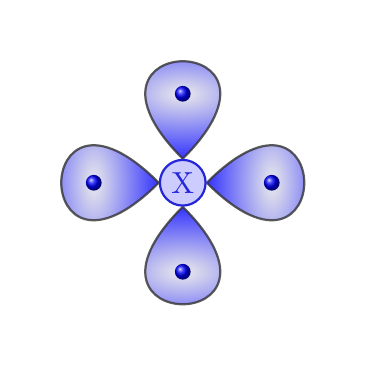
\begin{tikzpicture}
\atom[name=X, color=blue, scale = 1.1]{
blue/90/north/1,
blue/0/east/1,
blue/270/south/1,
blue/180/west/1}
\end{tikzpicture}
\quad \textrightarrow \quad
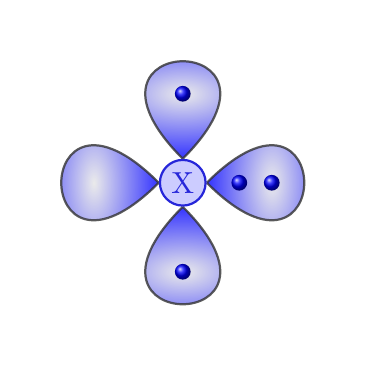
\begin{tikzpicture}
\atom[name=X, color=blue, scale=1.1]{
blue/90/north/1,
blue/0/east/2,
blue/270/south/1,
blue/180/west/0}
\end{tikzpicture}

An electronic transition can also be described by term symbols
\end{center}
}

\only<4>{
\begin{center}
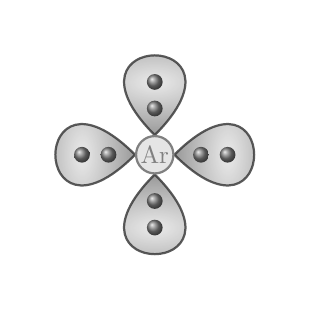
\begin{tikzpicture}
\atom[name=Ar, color=gray,scale = 0.9]{ 
gray/180/west/2,
gray/90/north/2,
gray/270/south/2,
gray/0/east/2}
\end{tikzpicture}
\end{center}

\medskip If the atom has completely filled subshells, then there are no alternative ways of arranging the electrons in the available orbitals. Therefore, \emph{Only \textbf{unfilled subshells} need to be considered when determining the appropriate \textbf{Term Symbols} for an atom or molecule}

\medskip The term symbols contain information on angular momenta and spin quantum number of atoms, or molecules. So first we have to deal with these angular momenta. 
}
\end{frame}

\subsection{Angular momenta and Spin-orbit interactions}

\begin{frame}
\frametitle{What is Angular momentum?}
\only<1>{Angular momentum is the rotational equivalent of linear momentum. \textit{Linear} momentum is the product of mass and linear speed, \(p = mv\). 

\bigskip Non-linear motion produces angular momentum. \textit{Angular} momentum \textit{L} is proportional to moment of inertia \textit{I} and angular speed \(\omega\). 
}
\only<2>{
\medskip In atoms, each electron has two kinds of motions producing angular momentum: \textbf{Orbital motion} and \textbf{spin motion}  

\begin{figure}[h]
\centering
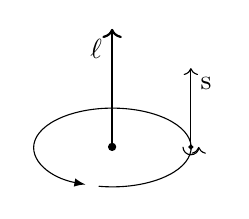
\begin{tikzpicture}
\draw[fill] (0,0) circle [radius=0.045];
%\draw (0,0) ellipse (1cm and 0.5cm);
\draw[thick, ->] (0,0) -- (0,1.5) node[anchor=north east] { \(\ell\)};
\draw[fill] (1,0) circle [radius=0.025];
\draw[->] (0.9,0) arc [start angle = -180, end angle = 0, x radius =0.1cm, y radius = 0.1cm];
\draw[thin, ->] (1,0) -- (1,1) node[anchor=north west] {s};
\draw [-latex, thin, rotate = 90] (-0.5,0.17) arc [start angle=-190, end angle=160, x radius=0.5cm, y radius=1cm];
\end{tikzpicture}
\caption{Angular momenta from orbital and spin motion. the angular momenta have \textit{direction} and \textit{magnitude}}
\end{figure}
}
\end{frame}

\begin{frame}
\frametitle{Total angular momentum for one electron}
\only<1>{
The \emph{magnitude} of \underline{orbital momentum vector} for a single electron is: 
\begin{equation} \label{angularmagnitude} [\ell(\ell+1)]^{1/2}\hbar \end{equation}
where \(\ell = 0,1,2,...,(n-1)\)  \par
\medskip
The \emph{magnitude} of the \underline{spin angular momentum vector} for a single electron is: \[ [s(s+1)]^{1/2} \hbar \]
where s = \(\frac{1}{2}\)
}
\only<2>{
So if one electron has two kinds of angular momentum, which are vector quantities, then it follows that there must be a resultant angular momentum that we can call the total angular momentum for that electron.\par

Like the two angular momenta, the total angular momentum has a \textit{direction} and a \textit{magnitude}.\par

\medskip The \emph{magnitude} of the \textbf{Total (orbital + spin) angular momentum}, \(\jmath\), is: \[ [\jmath(\jmath+1)]^{1/2}\hbar\]
where \(\jmath=\ell+s, \ell+s-1, \ldots, |\ell-s|\)  
\par\medskip
For one-electron atoms \(\jmath\) is not particularly useful, but \(J\) in polyelectronic atoms is very important.
}
\end{frame}

\begin{frame}
\frametitle{Magnetic moments}
An electron in orbit is like an electric current and produces a magnetic moment\newline\medskip
The magnetic moment due to orbital motion, \(\mu_\ell\), is a vector\newline\medskip
This is \underline{opposed} to the corresponding orbital angular momentum vector, \(\vec{\ell}\)\newline\medskip
Electron spin causes a magnetic moment, \(\mu_s\), associated with the spin angular momentum, \(s\).\newline\(\mu_s\) is opposed to \(s\). 
\(\mu_\ell\) and \(\mu_s\) act like tiny bar magnets. They may be parallell or opposed
\end{frame}

\begin{frame}
\frametitle{angular momenta and magnetic moments}
\only<1>{
\begin{figure}[h]
\centering
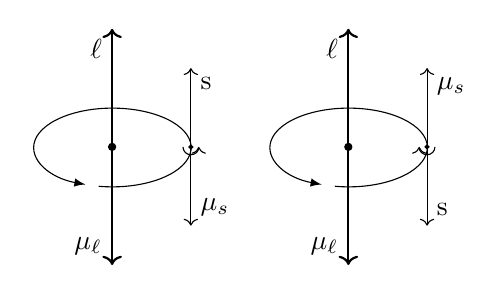
\begin{tikzpicture}
\draw[fill] (0,0) circle [radius=0.045];
%\draw (0,0) ellipse (1cm and 0.5cm);
\draw[thick, ->] (0,0) -- (0,1.5) node[anchor=north east] { \(\ell\)};
\draw[thick, ->] (0,0) -- (0,-1.5) node[anchor = south east] {\(\mu_\ell\)};
\draw[fill] (1,0) circle [radius=0.025];
%\draw  (1,0) ellipse (.1cm and 0.05cm);
\draw[->] (0.9,0) arc [start angle = -180, end angle = 0, x radius =0.1cm, y radius = 0.1cm];
\draw[thin, ->] (1,0) -- (1,1) node[anchor=north west] {s};
\draw[thin, ->] (1,0) -- (1,-1) node[anchor = south west] {\(\mu_s\)};
%\draw[thin,->] (-1,0) -- (-1,-0.01);
\draw[fill] (3,0) circle [radius=0.045];
%\draw (3,0) ellipse (1cm and 0.5cm);
%\draw[thin,->] (2,0) -- (2,-0.01);
\draw[thick, ->] (3,0) -- (3,1.5) node[anchor=north east] { \(\ell\)};
\draw[thick, ->] (3,0) -- (3,-1.5) node[anchor = south east] {\(\mu_\ell\)};
\draw[fill] (4,0) circle [radius=0.025];
%\draw (4,0) ellipse (.1cm and 0.05cm);
\draw[->] (4.1,0) arc [start angle = 0, end angle = -180, x radius =0.1cm, y radius = 0.1cm];
\draw[thin, ->] (4,0) -- (4,1) node[anchor=north west] {\(\mu_s\)};
\draw[thin, ->] (4,0) -- (4,-1) node[anchor = south west] {s};

\draw [-latex, thin, rotate = 90] (-0.5,0.17) arc [start angle=-190, end angle=160, x radius=0.5cm, y radius=1cm];
\draw [-latex, thin, rotate = 90] (-0.5,-2.83) arc [start angle=-190, end angle=160, x radius=0.5cm, y radius=1cm];
\end{tikzpicture}
\caption{angular momenta and magnetic moments}
\end{figure}
}

\only<2>{
\begin{description}
\item[\(\ell\)] orbital angular momentum
\item[\(s\)] spin angular momentum
\item[\(\mu_\ell\)] orbital magnetic momentum
\item[\(\mu_s\)] spin magnetic momentum
\end{description}
}
\end{frame}

%\section{Terms and term symbols}
\section{Atomic Terms and Term Symbols}
\subsection{Single-electron atoms}

\begin{frame}
\frametitle{Term symbols for single electron atoms}
The term expression is given by \(^{2S+1}L_J\) \newline

\bigskip In this expression, S is the total spin (which is always equal to 1/2), L is the orbital angular momentum (for single electron equal to \(\ell\)).\newline

\medskip The symbols corresponding to the possible values of L (= 0,1,2,3,4,...) are S, P, D, F, G, ...\newline

\medskip This means that for Hydrogen, with one electron, the spin \(s=1/2\) and \(\ell=0\), the Term Expression is given by s=1/2 and \(\ell=0\) and \(\jmath = 1/2 + 0\). \newline

\medskip The Term symbol for the H-atom is therefore:
\[^{2S+1}L_J = ^{2s+1}\ell_\jmath = ^{2/2 + 1}0_{1/2} \implies ^2S_{1/2}\]
\end{frame}

\begin{frame}
\frametitle{Term symbols for atoms}
\begin{itemize}
%\item Described by the primary quantum number n
\item The angular momentum quantum number L
\item Spin quantum number S
\item Total angular momentum quantum number J
\end{itemize}

\bigskip The term symbol becomes \[ ^{2S+1}L_J\]
\end{frame}

\subsection{Multi-electron atoms}

\begin{frame}
\frametitle{Many-electron atoms}
\only<1>{
Having more than one electron in an atom raises the issues of the indistinguishability of electrons, the electron spin, and the interaction between orbital and spin magnetic moments. 

\medskip Taking these issues into consideration leads to a new set of quantum numbers for the states of many-electron atoms and the groupings of these states into levels and terms. 
}

\only<2>{
Remember that a configuration specifies only the \textit{n} and \(\ell\) values for the electrons and not the \(m_\ell\) and \(m_s\) values.

\medskip For many atoms, the configuration does not completely define the quantum state. 

\medskip Under what circumstances do the values of \(m_\ell\) and \(m_s\) for a given configuraiton lead to different spatial distributions of electrons and therefore to a different electron-electron repulsion?

\medskip This occurs when there are at least two electrons in the valence shell and then there are multiple choices in \(m_\ell\) and \(m_s\) for these electrons consistent with the Pauli principle and the configuration.
}

\only<3>{
This is not the case for the ground states of the rare gases, the alkali metals, the alkaline earth metals, group III and the halogens. 

\medskip Atoms in all of these groups have either a filled shell or subshell or only one electron or one electron fewer than the maximum number of electrons in a subshell. 

\medskip None of these atoms has more than one unpaired electron in its ground state and all are uniquely described by their configuration

\medskip However, the ground states for carbon, nitrogen and oxygen are not completely described by a configuration.
}

\only<4>{
Several quantum states, all of which are consistent with the configuration, have significantly different values for the total energy as well as different chemical reactivities.

\medskip For atoms with Z \(<\) 40, the total energy is essentially independent of \(M_L\) and \(M_S\)

\medskip Therefore, a group of different quantum states that have the same values for L and S but different values of \(M_L\) and \(M_S\) is degenerate in energy

\medskip Such a group of states is called a \textit{term}, and the L and S values for the term are indicated by the \textbf{term symbol} \(^{(2S+1)}L\)
}

\only<5>{
Because there are 2L + 1 quantum states (different \(M_L\) values) for a given value of L and 2S + 1 states (diferent \(M_S\) values) for a given value of S, a term will include (2L + 1)(2S + 1) quantum states, all with the same energy to a good approximation

\medskip This is the \textbf{degeneracy of a term}. The superscript 2S + 1 is called the \textbf{multiplicity}, and the words \textit{singlet} and \textit{triplet} refer to 2S + 1 = 1 and 3, respectively.

\medskip For a filled subshell or shell,
\[ M_L = \sum_i m_{li} = M_S = \sum_i m_{si} = 0\]

and \(M_L = 0\) and \(M_S = 0\) are only consistent with L = 0 and S = 0
}

\only<6>{
Therefore all atoms with no unpaired electrons that have either a filled valence subshell or shell are characterised by the term \(^1S\)

\medskip Note that the term symbol does not depend on the principal quantum number of the valence shell

\medskip Carbon, which has the \(1s^22s^22p^2\) configuration, has the same set of terms as silicon, which has the \(1s^22s^22p^63s^23p^2\) configuration.
}
\end{frame}


Atomic spectroscopies give information on the discrete energy levels of an atom and provide the basis for understanding the coupling of the individual spin and orbital angular momentum vectors in a many-electron atom. Because the discrete energy levels for atoms differ, atomic spectorscopies give information on the identity and concentration of atoms in a sample. For this reason, atomic spectroscopies are widely used in analytical chemistry. The discrete energy spectra of atoms and the difference in rates of transition between quantum states can be used to construct lasers that provide and intense and coherent source of monochromatic radiation. Atomic spectroscopies can also provide elemental identification specific to the first fewa atomic layers of a solid. The reactions of electronically excited atoms can differ dramatically from their ground-state counterparts, as evidenced by reactions in Earth's atmosphere.

\begin{frame}
\frametitle{Multi-electron atoms}
\only<1>{
For many-electron atoms it is not convenient to reel off a list of properties for each electron to describe the atom. So we need to combine the quantum numbers from multiple electrons into another set of quantum numbers that describe the entire \emph{atom}.\par

\medskip A useful model to describe atoms with atomic number, \(Z < 40\), is to form vector sums of their orbital and spin angular momenta separately. \par
}

\only<2>{
This generates the total orbital and spin momentum vectors \textbf{L} and \textbf{S} \mode<article>{(Figure \ref{vectorsum})} 

\begin{equation}\label{totalsLS} L = \sum_i \ell_i \hspace{1cm} S = \sum_i s_i\end{equation}

Remember, only electrons in unfilled subshells contribute to these sums.
}

\only<3>{
\begin{figure}[h]
\centering
%\setlength{\unitlength}{1cm}
\begin{picture}(100,100)(0,0)
\thicklines
\put(10,0){\vector(0,1){45}}
\put(10,45){\vector(1,1){42}}
\put(10,0){\vector(1,2){45}}
\put(0,20){\(\ell_1\)}
\put(20,65){\(\ell_2\)}
\put(30,30){L}
\end{picture}
\caption{Vector addition of angular momenta, \(\ell\)}
\label{vectorsum}
\end{figure}
}

\only<4>{
The quantum number \textbf{L} is associated with the total orbital angular momentum for the two electrons.\par

L can take on the values:\newline
\[L = \ell_1 + \ell_2, \ell_1 + \ell_2 - 1, \ell_1 + \ell_2 - 2, ..., |\ell_1 - \ell_2|\]

\bigskip The \textbf{Term Symbols} are given by the values of L:
\begin{tabular}{cc}
L & Term Symbol\\\hline
0 & S\\
1 & P\\
2 & D\\
3 & F\\
4 & G\\\hline
\end{tabular}

\bigskip Note that for \emph{filled subshells}, e.g. \(2p^6\) or \(3d^{10} \implies L=0\)
}

\only<5>{
\begin{align*}
L&=\sum_i\ell_i & S&=\sum_is_i\\
M_L &= \sum_{i=1}^n m_{\ell_i} & M_S &= \sum_{i=1}^n m_{s_i}
\end{align*}

\bigskip \(M_L\) and \(M_S\) are the scalar values of the z-components of the L and S vectors

%add illustration here
}
\end{frame}

\begin{frame}
\frametitle{Good quantum numbers}
\only<1>{
How do we assign quantum numbers to many-electron atoms?

\medskip The quantum numbers \(n,\ \ell,\ m_\ell\) and \(m_s\) that were used for the H atom are \textbf{good quantum numbers} for H, but they are not good quantum numbers for many-electron atoms or ions.

\medskip Another set of good quantum numbers must be found.

\medskip Good quantum numbers are generated by forming vector sums of the electronic orbital and spin angular momenta separately, \textbf{L} and \textbf{S}, which have z-components \(M_L\) and \(M_S\), respectively
}

\only<2-4>{
Only electrons in unfilled subshells contribute to these sums:

\begin{center} \(L = \sum_i\ell_i\) \qquad \(S = \sum_is_i\)\end{center}

where the summation is over the electrons in unfilled subshells.
}

\visible<3->{
\bigskip Just like \(\ell\) for the single-electron atoms, the \textit{magnitudes} of \textbf{L} and \textbf{S} are \(\sqrt{L(L+1)}\hbar\) and \(\sqrt{S(S+1)}\hbar\)
}

\visible<4>{
\bigskip The good quantum numbers for many-electron atoms for Z\(<\)40 are \(L,\ S,\ M_L\) and \(M_S\).
}
\end{frame}

\begin{frame}
\includegraphics[width=\textwidth]{../../graphics/cones}
\end{frame}

\subsubsection{Multiplicity}

\begin{frame}{Multiplicity}
\only<1>{
Multiplicity is the number of values M\(_S\) can take.
\[M_S = S, S-1, ..., -S\]

\par For a filled orbital: \(M_S = \sum_i(m_s)_i = 0\) \mode<article>{(from equation \ref{totalsLS})} \(\implies S=0\)
}

\only<2>{
\begin{example}{Excited configurations of C and Si}\par\medskip
C: \(1s^22s^22p^13d^1\)\newline

Si: \(1s^22s^22p^63s^23p^13d^1\) \newline
\par These will produce P, D and F terms like the excited configuration of He\(^*\) we saw above.\par
\medskip But because of multiplicity there will be both singlet and triplet terms:\newline
\[^1P,\ ^3P,\ ^1D,\ ^3D,\ ^1F,\ ^3F\]
\par The superscript before the term symbol indicates the \textit{Multiplicity}
\end{example}
}
\end{frame}

\begin{frame}
\frametitle{Atomic Terms}
\begin{definition}[Term]
A group of quantum states with same value of L and S but different values of \(M_L\) and \(M_S\) are degenerate in energy, and called a \emph{Term}
\end{definition}
An atomic Term is described by
\[ ^{2S+1}L\] where L = 0,1,2,3,... corresponding to term symbols S, P, D, F, G
\end{frame}

\lecture[Lecture 4]{Configurations, states and terms}{Lecture 4}

\subsection{Configurations, terms, levels and states}

\begin{frame}
\frametitle{Configuration - term - level - state}
\only<1>{
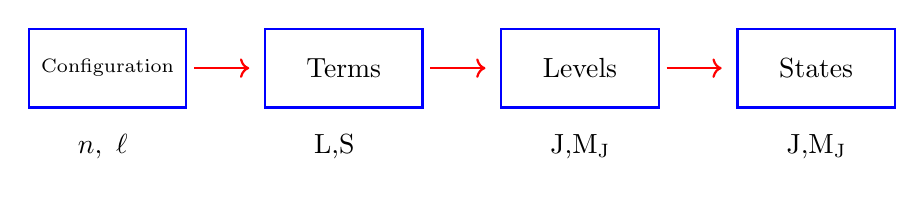
\begin{tikzpicture}
%\draw[help lines] (0,0) grid (12,5);
\draw[blue, thick] (0,2) rectangle (2,3);
\node[right] at (0.5,1.5) {\(n,\ \ell\)};
\node at (1,2.5) {\scriptsize Configuration};
\draw[->,red,thick] (2.1,2.5) -- (2.8,2.5);
\draw[blue,thick] (3,2) rectangle (5,3);
\node[right] at (3.5,1.5) {L,S};
\node at (4,2.5) {Terms};
\draw[->,red,thick] (5.1,2.5) -- (5.8,2.5);
\draw[blue,thick] (6,2) rectangle (8,3);
\node[right] at (6.5,1.5) {J,M\textsubscript{J}};
\node at (7,2.5) {Levels};
\draw[->,red,thick] (8.1,2.5) -- (8.8,2.5);
\draw[blue,thick] (9,2) rectangle (11,3);
\node[right] at (9.5,1.5) {J,M\textsubscript{J}};
\node at (10,2.5) {States};
\end{tikzpicture}
}

\only<2>{
\begin{description}
\item[Configuration:] a gross but useful approximation. Electron fed into orbitals of energies calculated without the last term in eq. 7.2 (Holles)
\item[State:] Most configurations give rise to more than one state. Observable experimentally
\item[Term:] approximate treatment of electron configuration
\end{description}

\begin{plainbox}
Example: a \(^3P\) term splits into \( ^3P_1,\ ^3P_2,\) and \(^3P_3\) states
\end{plainbox}
}

\end{frame}


\begin{frame}
\frametitle{configuration and quantum states}

\begin{alertblock}{configuration and quantum states}
\alert{configuration} is the specific value of n and \(\ell\)\newline
Rare gases, alkali metals, alkaline earth group III and halogens are all completely described by their configuration. Other elements have multiple quantum states arising from different possible combinations of \(m_l\) and \(m_s\) consistent with their configuration, with different energies and chemical reactivity
\end{alertblock}

The ground states are not completely described by the configuration.  

Several quantum states are consistent with the configuration, with different energies and chemical reactivity.
\end{frame}


\subsection{Coupling of Angular Momenta in multi-electron atoms}

\begin{frame}
\frametitle{Coupling of angular momenta}
Momenta interact with each other.\newline\bigskip
The stronger the momentum, the stronger the interaction (called coupling)

Spin-orbit coupling is the interaction between the spin of one electron with i) the spins of other electrons, ii) its own orbital motion and iii) orbital motions of other electrons. Sometimes one of these types of interactions is the dominant one and it can be assumed that the other types have negligible contributions.
\par\bigskip
Spin-Orbit coupling approximation regimes:
\begin{itemize}
\item \textit{jj}-coupling 
\item \(\ell\ell\)-coupling 
\item \(ss\)-coupling
\item LS-coupling
\end{itemize}
\end{frame}

\subsubsection{jj-coupling}
\begin{frame}
\frametitle{\textit{jj}-coupling}
Spin momenta (i) coupling is too weak and orbital momenta coupling too weak. 

\medskip But the spin of electron 1 and angular momentum of electron 1 are strong enough to be appreciable. 

\medskip The interactions between the \textit{j}s of the electrons are appreciable
\end{frame}

\subsubsection{\(\ell\ell\)-coupling}
\begin{frame}
\frametitle{\(\ell\ell\)-coupling}
\only<1>{
This neglects the coupling between the spin on electron 1 and its orbital angular momentum. Assumes strong interaction between orbital momenta. Assumes appreciable interaction between spin momenta. 

\bigskip When you have non-equivalent electrons (different n or \(\ell\)), consider strong coupling between orbital angular momenta (\(\ell\ell\)-coupling).\newline

\medskip For example, the He atom \(2p^13d^1\) configuration (highly excited). This gives rise to P, D and F-terms (see below for explanation).

\medskip For this configuration, the values of \(\ell_1 = 1\) and \(\ell_2 = 2\). \par
}

\only<2>{
\medskip This means their magnitudes are \mode<article>{given by equation \ref{angularmagnitude} as} \(2^{\frac{1}{2}}\hbar\) and \(6^{\frac{1}{2}}\hbar\)

The magnitude of the vector sum \mode<article>{is also given by equation \ref{angularmagnitude},} subsituting L for \(\ell\): \([L(L+1)]^{\frac{1}{2}}\hbar\)\par

\medskip So the relative orientations of \(\ell_1\) and \(\ell_2\) are restricted by the values that L can take. The resultant vector \(\overrightarrow{L}\) has to be the same as the sum of the vectors \(\overrightarrow{\ell_1}\) and \(\overrightarrow{\ell_2}\)\par
\medskip This is the kind of thing we encounter in \emph{quantum} chemistry. Things are \emph{quantized}!
}
\end{frame}

\begin{frame}{Vector quantities added}
\only<1>{
For a \(2p^13d^1\) configuration then, the possible values for L are \textbf{3, 2 and 1}\par
\medskip This means the possible \emph{magnitudes} of L are \(12^{\frac{1}{2}}\hbar\), \(6^{\frac{1}{2}}\hbar\) and \(2^{\frac{1}{2}}\hbar\)\par

\begin{figure}[h]
\centering
\begin{picture}(200,150)
\thicklines
\put(10,0){\vector(0,1){90}}
\put(10,90){\vector(1,1){48}}
\put(10,0){\vector(1,3){45}}
\put(0,20){\(\ell_1\)}
\put(20,110){\(\ell_2\)}
\put(30,30){L=3}
\put(0,-10){an F-term}

\put(100,0){\vector(0,1){90}}
\put(100,90){\vector(2,-1){38}}
\put(100,0){\vector(1,2){38}}
\put(90,20){\(\ell_1\)}
\put(110,90){\(\ell_2\)}
\put(120,30){L=2}
\put(90,-10){a D-term}

\put(190,0){\vector(0,1){90}}
\put(190,90){\vector(1,-2){23}}
\put(190,0){\vector(1,2){23}}
\put(180,20){\(\ell_1\)}
\put(200,80){\(\ell_2\)}
\put(210,20){L=1}
\put(180,-10){a P-term}
\end{picture}
\caption{Allowed orientations of total angular momentum vector}
\label{totalangular}
\end{figure}
}

\only<2>{
\includegraphics[width=.8\textwidth]{../../graphics/spacequant}
}
\end{frame}

\begin{frame}
\frametitle{Space quantization of orbital angular momentum}
\only<1>{
\par Space quantization of the total orbital angular momentum\\ produces 2L + 1 components:
\[ M_L = L, L-1, L-2, ..., -L\]
\par This is analogous to the space quantiation of \(\ell\) and the possible orientations given by the possible values of \(m_\ell\).
}

\only<2-3>{
\begin{tikzpicture}
%\draw[help lines] (0,0) grid (12,5);
\draw[->,thick] (2,0) -- (0,5);
\node at (0.5,1.5) {L};
\draw[->] (2,0) -- (4,2);
\node at (3.5,0.5) {\(\ell_1\)};
\draw[->] (4,2) -- (2,2.5);
\node at (3,2.5) {\(\ell_2\)};
\draw[->] (2,2.5) -- (0,5);
\node at (2,3.5) {\(\ell_3\)};
\draw[dashed] (2,0) -- (5,0);
\draw[dashed] (4,2) -- (5,2);
\draw[dashed] (2,2.5) -- (5,2.5);
\draw[dashed] (0,5) -- (5,5);
\draw[->] (5,0) -- (5,6);
\node[above] at (5,6) {L\textsubscript{z}};
\draw[<->] (6,0) -- (6,2);
\draw[<->] (6,2) -- (6,2.5);
\draw[<->] (6,2.5) -- (6,5);
\node at (6.5,1) {\(\ell_{1z}\)};
\node at (6.5,2.2) {\(\ell_{2z}\)};
\node at (6.5,3.5) {\(\ell_{3z}\)};
\visible<3>{
\draw[->,thick] (7,0) -- (7,5);
\node at (7.5,2.5) {\textbf{M\textsubscript{L}}};
}
\end{tikzpicture}
}

\only<4>{
Only the length of an angular momentum vector and one of its components can be known in quantum mechanics, and we choose the z-direction.

\medskip To find the sum M\textsubscript{L} the known components \(\ell_{zi}\) add as scalars, \(M_L = \sum_i \ell_{zi}\)
}
\end{frame}

\subsubsection{ss-coupling}
\begin{frame}
\frametitle{\(ss\)-coupling}
In ss-coupling we know that the spin, \textit{s}, is always \(\frac{1}{2}\), so the vector for each electron is always of magnitude \(3^{\frac{1}{2}}\frac{\hbar}{2}\) \mode<article>{(from equation \ref{angularmagnitude})}\par

\medskip Two s-vectors can only take up orientations such that the resultant \textbf{S} is of magnitude:
\[[s(s+1)]^{^1/_2}\hbar\]
where S is total spin quantum number:\newline
\begin{equation} \label{totalspin} S = s_1 + s_2, s_1 + s_2 -1, s_1 + s_2 - 2, ..., |s_1 - s_2|\end{equation}

For two electrons: S = 0 or S =1\newline

\begin{figure}[h]
\centering
\begin{picture}(100,60)
\thicklines
\put(10,10){\vector(0,1){40}}
\put(30,50){\vector(0,-1){40}}
\put(0,20){\(s_1\)}
\put(40,20){\(s_2\)}
\put(10,0){S = 0}

\put(80,10){\vector(0,1){40}}
\put(80,50){\vector(1,-1){20}}
\put(80,10){\vector(1,1){20}}
\put(70,20){\(s_1\)}
\put(90,50){\(s_2\)}
\put(90,10){S (magnitude = \(2^{^1/_2}\hbar\))}
\put(80,0){S = 1}
\end{picture}
\end{figure}

\end{frame}

\begin{frame}
\frametitle{Quantization of spin angular momentum}
\only<1>{
As we've seen, spin angular momentum, \(\vec{s}\) has the magnitude \(|s| = \sqrt{s(s+1)}\hbar\)

\medskip For a configuration like \(1s^12s^1\) (He), \(\vec{s}\) has 2s+1 = 2 possible orientations, because s=1/2

\bigskip We add the scalar components \(m_s\) for the two electrons in each of the four possible combinations, \(M_S = m_{s1} + m_{s2}\implies \) 0,0,-1,+1\newline

\medskip\(S\ge|M_S|\) \qquad \(M_S = \pm 1 \implies S=1\)\newline

\medskip \(M_S = S, S-1, ..., -S\)
}

\only<2>{
so \(M_S\) takes on all integral values between +S and -S, so the S=1 group must include \(M_S=\) 0,+1 and -1

\medskip The remaining combination has \(M_S=0\), which is only consistent with S=0

\medskip Three of four possible combinations are characterised by S=1, with \(M_S=\pm1\) and the fourth has S=0 with \(M_S=0\)

\medskip The S=0 spin combination is a singlet, the S=1 combination is a triplet
}

\only<3>{
\medskip So to reiterate: \(M_L\) and \(M_S\) are the scalar values of the z-components of the L and S vectors

\medskip and the quantum numbers we use for many-electron atoms are \(L,\ S,\ M_L\) and \( M_S\)
}
\end{frame}


\subsubsection{LS-coupling}

\begin{frame}
\frametitle{LS-coupling}
\only<1>{
Also called \textbf{Russell-Saunders approximation}. This is the coupling between the \textit{resultant orbital} and \textit{resultant spin} momenta.\newline
\medskip Due to spin-orbit interaction caused by positive charge Ze on the nucleus \(\approx Z^4\)\newline
\medskip Coupling between L and S (vectors) given the total angular momentum vector, J\newline

\medskip J has magnitude: \hspace{1.5in} \([J(J+1)]^{^1/_2}\hbar\)

\medskip and can take on the values:  \hfill \(J = L+S, L+S-1, ..., |L-S|\)

\medskip if \(L>S \implies\) J can take 2S+1 values\newline
\medskip if \(L<S \implies\) J can take 2L+1 values
}

\only<2>{
\begin{center}\includegraphics[width=.5\textwidth]{../../graphics/LScoupling}\end{center}
}

\only<3>{
\begin{example}{LS coupling in a \(^3D\) term}
\begin{figure}[h]
\centering
\begin{picture}(200,150)
\thicklines
\put(10,0){\vector(0,1){90}}
\put(10,90){\vector(1,1){48}}
\put(10,0){\vector(1,3){45}}
\put(0,20){L}
\put(20,110){S}
\put(30,30){J = 3}
\put(0,-10){\(^3D_3\)}

\put(100,0){\vector(0,1){90}}
\put(100,90){\vector(2,-1){38}}
\put(100,0){\vector(1,2){38}}
\put(90,20){L}
\put(110,90){S}
\put(120,30){J = 2}
\put(90,-10){\(^3D_2\)}

\put(190,0){\vector(0,1){90}}
\put(190,90){\vector(1,-2){23}}
\put(190,0){\vector(1,2){23}}
\put(180,20){L}
\put(200,80){S}
\put(210,20){J =  1}
\put(180,-10){\(^3D_1\)}
\end{picture}
\caption{S=1 and L=2 \(\implies\) J = 3, 2 or 1. }
\label{LScoupling}
\bigskip The term expression is given by \(^{2S+1}L_J\) !
\end{figure}
\end{example}
}

\only<4>{
\begin{titleplainbox}{The total number of states arising from the C or Si configuration:}
\(^1P_1,\ ^3P_0,\ ^3P_1,\ ^3P_2,\ ^1D_2,\ ^3D_1,\ ^3D_2,\ ^3D_3,\ ^1F_3,\ ^3F_2,\ ^3F_3,\ ^3F_4\)
\end{titleplainbox}
}
\end{frame}

\lecture[Lecture 5]{Term symbols for ground states and Hund's rules}{Lecture 5}

\subsubsection{Equivalent electrons}
\begin{frame}
\frametitle{What are equivalent electrons?}

These are electrons with the same values of n and \(\ell\)\newline
\end{frame}

\begin{frame}
\frametitle{Carbon}
\only<1>{The ground configuration of Carbon:

C : \quad \(1s^22s^22p^2\)\newline
\medskip only the 2p electron must be considered (remember filled subshells!)\newline

\medskip Both electrons: n = 2 and \(\ell\) = 1. This means they \emph{must} have different values of \(m_\ell\) or \(m_s\).\newline

\medskip 
\(\ell_1 = 1\) \((m_\ell)_1 = +1,0,-1\) \quad \(\ell_2=1\) \((m_\ell)_2 = +1,0,-1\)\par
\medskip \(s_1 = \frac{1}{2}\) \((m_s)_1 = +\frac{1}{2}, -\frac{1}{2}\) \quad \(s_2 = \frac{1}{2}\) \((m_s)_2 = \pm \frac{1}{2}\)\newline
}

\only<2>{
\medskip
There are 3x2 combinations of \((m_\ell)_1\) and \((m_s)_1\)\par

\medskip There are 3x2 - 1 combinations of \((m_\ell)_2\) and \((m_s)_2\) (due to the Pauli exclusion principle)\\

\medskip This means that there are 6x5 = 30 combinations for \(e_1\) and \(e_2\). \\

\medskip
BUT, the electrons are indistinguishable. if they swapped positions it wouldn't matter, so the number of combinations is only half of that, i.e. 15 !
}

\only<3>{
\begin{example}{Carbon terms}
\newline 1. Calculate possible values for \(M_L = \sum_i m_{\ell_i}\) and \(M_S=\sum_i m_{s_i}\)
\newline 2. what values of L and S are consistent with the \(M_S\) and \(M_L\) given that \(-L \leq M_L \leq L\) and \(-S \leq M_S \leq S\)\newline

each term has (2S+1)(2L+1) states associated with it
\end{example}
}

\only<4>{
States and terms for the \(np^2\) configuration\newline
\resizebox{\textwidth}{!}{
\begin{tabular}{ccccccc}
\(m_{\ell_1}\) & \(m_{\ell_2}\) & \(M_L = m_{\ell_1} + m_{\ell_2}\) & \(m_{s_1}\) & \(m_{s_2}\) & \(M_S = m_{s_1} + m_{s_2}\) & Term \\\hline\hline

-1 & -1 & -2 & 1/2 & 1/2 & 0 & \(^1D\)\\\hline
0 & -1 & -1 & -1/2 & -1/2 & -1 & \(^3P\)\\
0 & -1 & -1 & -1/2 & 1/2 & 0 & \(^1D,\ ^3P\)\\
0 & -1 & -1 & 1/2 & -1/2 & 0 & \(^1D,\ ^3P\)\\
0 & -1 & -1 & 1/2 & 1/2 & 1 & \(^3P\)\\\hline
0 & 0 & 0 & 1/2 & -1/2 & 0 & \(^1D,\ ^3P,\ ^1S\)\\
1 & -1 & 0 & -1/2 & 1/2 & 0 & \(^1D,\ ^3P,\ ^1S\)\\
1 & -1 & 0 & 1/2 & -1/2 & 0 & \(^1D,\ ^3P,\ ^1S\)\\
1 & -1 & 0 & -1/2 & -1/2 & -1 & \(^3P\)\\
1 & -1 & 0 & 1/2 & 1/2 & 1 & \(^3P\)\\\hline
1 & 0 & 1 & -1/2 & -1/2 & -1 & \(^3P\)\\
1 & 0 & 1 & -1/2 & 1/2 & 0 & \(^1D,\ ^3P\)\\
1 & 0 & 1 & 1/2 & -1/2 & 0 & \(^1D,\ ^3P\)\\
1 & 0 & 1 & 1/2 & 1/2 & 1 & \(^3P\)\\
1 & 1 & 2 & 1/2 & -1/2 & 0 & \(^1D\)\\\hline\hline
\end{tabular}}
}

\only<5>{
If \(M_L = \pm 2\), they must belong to a term with L=2 (a D-term)\newline

All states with \(M_L = \pm 2\) have \(M_S=0\)\par

\medskip If \(m_{\ell_1} = m_{\ell_2} \implies m_{s_1} \neq m_{s_2}\)\par

\medskip So S=0 and 2S+1 = 1, so it is a \(^1D\)-term.\par

\medskip There are (2S+1)(2L+1) = 5 states for this term.
}

\only<6>{
This \(^1D\) term includes states with \(M_L\) = -2,-1,0,+1 and +2, all of which have \(M_S=0\)

\medskip Taking 5 states out of the table leaves us with 10 sttes.

\medskip The highest value of \(M_L\) of those remaining is +1, which must belong to a P-term.

\medskip Because there is a combination of with \(M_L=1\) and \(M_S=1\), the P-term must be \(^3P\)
}

\only<7>{
The \(^3P\)-term has (2S+1)(2L+1) = 9 states associated with it and taking those out of the table leaves one single state with \(M_L = M_S = 0\). This is a complete \(^1S\) term

\medskip By elimination we have found that the 15 combinations of \(m_\ell\) and \(m_s\) consistent with the configuration \(1s^22s^22p^2\) separate into \(^1D\), \(^1S\) and \(^3P\) terms.

\medskip This is true for \textit{any} \(np^2\) configuration
}
\end{frame}

\begin{frame}
\frametitle{Other examples}
\only<1>{
Look at Helium in the excited state \(2p^13d^1\):\par

\medskip In this state, \(\ell_1 = 1\) and \(\ell_2=2\) so L = 1+2, 1+2-1, ..., \(|\)1-2\(|\)\par

\medskip This gives the possible values L = 3,2,1 which correspond to P D and F-terms\par
}

\only<2>{
The same situation is true for Carbon and silicon in the excited states:\par

\medskip \(C^*\): \(1s^22s^22p^13d^1\) \hspace{1in} P, D, F\par
\(Si^*\): \(1s^22s^22p^63s^23p^13d^1\) \hspace{3.7em} P D, F\newline

\medskip \(S= s_1 + s_2, s_1 + s_2 - 1, ... , |s_1 - s_2| \implies S=1,\ 0\)\par

\medskip \underline{S = 1, 0:}\par
S = 1: \(M_S = S, S-1, .. , -S = 1, 0, -1\), \quad 2S+1 = 3, 1\par
S = 0: \(M_S = 0\) \quad 2S+1 = 1\par

\medskip \(\implies ^1P,\ ^3P,\ ^1D,\ ^3D,\ ^1F,\ ^3F\) terms
}

\only<3>{
Li molecular terms: The Configuration is \(1s^22s^1\)\newline

\medskip n = 2: \(\ell\) = 0 \(\implies m_\ell = 0\)\newline \quad \(\ell = 1,0 \implies m_\ell = +1,0,-1\)\par

Reminder: n is the shell, orbitals with the same value of n and \(\ell\) are \textit{subshells}
}
\end{frame}

\subsubsection{Terms symbols for Ground state: Hund's rules}

\begin{frame}
\frametitle{Energy of terms}
\begin{alertblock}{Hund's Rules}
\begin{description}
\item[Rule 1] The lowest energy term is that which has the greatest spin multiplicity
\item[Rule 2] For terms with equal multiplicity the term with the greatest orbital angular momentum lies lowest in energy
\item[Rule 3] The order in energy of levels in a term:
\begin{itemize}
\item If unfilled subshells is half full or more, the level with highest J value (total angular momentum of an atom) is lower in energy
\item If unfilled subshell is less than half full, the level with lowest J value is lower in energy
\end{itemize}
\end{description}
\end{alertblock}
\end{frame}

\begin{frame}
\begin{center}\resizebox{!}{3.2in}{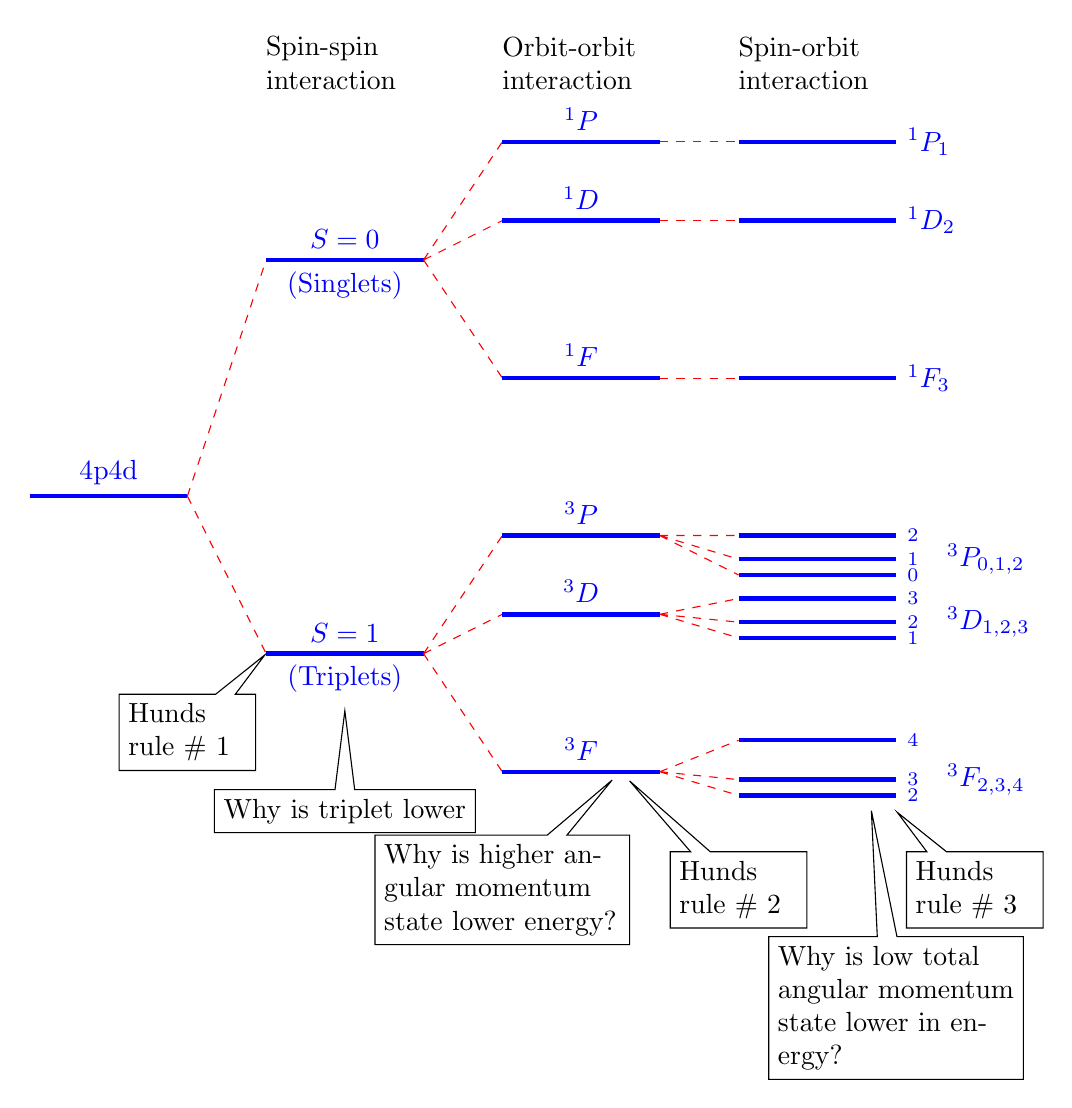
\begin{tikzpicture}
   % Draw all levels
  \draw[level] (0,0) -- node[above] {4p4d} (2,0);

  \draw[connect] (2,0)  -- (3,-2) (2,0) -- (3,3);
  \draw[level]   (3,3)  -- node[above] {$S=0$} node[below] {(Singlets)} (5,3);
  \draw[level]   (3,-2) -- node[above] {$S=1$} node[below] {(Triplets)} (5,-2);

  \draw[connect] (5,3)    -- (6,4.5) (5,3) -- (6,3.5) (5,3) -- (6,1.5);
  \draw[connect] (5,-2)   -- (6,-0.5) (5,-2) -- (6,-1.5) (5,-2) -- (6,-3.5);
  \draw[level]   (6,4.5)  -- node[above] {${}^1P$} (8,4.5);
  \draw[level]   (6,3.5)  -- node[above] {${}^1D$} (8,3.5);
  \draw[level]   (6,1.5)  -- node[above] {${}^1F$} (8,1.5);
  \draw[level]   (6,-0.5) -- node[above] {${}^3P$} (8,-0.5);
  \draw[level]   (6,-1.5) -- node[above] {${}^3D$} (8,-1.5);
  \draw[level]   (6,-3.5) -- node[above] {${}^3F$} (8,-3.5);

  \draw[connect] (8,4.5) -- (9,4.5) (8,3.5) -- (9,3.5) (8,1.5) -- (9,1.5);
  \draw[level]   (9,4.5) -- (11,4.5) node[right] {${}^1P_1$};
  \draw[level]   (9,3.5) -- (11,3.5) node[right] {${}^1D_2$};
  \draw[level]   (9,1.5) -- (11,1.5) node[right] {${}^1F_3$};

  \draw[connect] (8,-0.5) -- (9,-0.5) (8,-0.5) -- (9,-0.8) (8,-0.5) -- (9,-1)
                 (8,-1.5) -- (9,-1.6) (8,-1.5) -- (9,-1.8) (8,-1.5) -- (9,-1.3)
                 (8,-3.5) -- (9,-3.8) (8,-3.5) -- (9,-3.6) (8,-3.5) -- (9,-3.1);
  \foreach \i/\j in {2/-0.5, 1/-0.8, 0/-1} {
    \draw[level] (9,\j) -- (11,\j) node[right] {\scriptsize $\i$};
  }
  \node[level, right] at (11.5,-0.8) {${}^3P_{0,1,2}$};
  \foreach \i/\j in {3/-1.3, 2/-1.6, 1/-1.8} {
    \draw[level] (9,\j) -- (11,\j) node[right] {\scriptsize $\i$};
  }
  \node[level, right] at (11.5,-1.6) {${}^3D_{1,2,3}$};
  \foreach \i/\j in {4/-3.1, 3/-3.6, 2/-3.8} {
    \draw[level] (9,\j) -- (11,\j) node[right] {\scriptsize $\i$};
  }
  \node[level, right] at (11.5,-3.6) {${}^3F_{2,3,4}$};

  % Draw labels
  \node[label] at (4,5.5)  {Spin-spin interaction};
  \node[label] at (7,5.5)  {Orbit-orbit interaction};
  \node[label] at (10,5.5) {Spin-orbit interaction};

  % Draw annotations
  \node[notice={(0.5,0.5)}, text width=1.5cm] at (2,-3) {Hunds rule \# 1};
  \node[notice={(0,1)}] at (4,-4) {Why is triplet lower};
  \node[notice={(0.7,0.7)}, text width=3cm] at (6,-5)
    {Why is higher angular momentum state lower energy?};
  \node[notice={(-0.9,0.9)}, text width=1.5cm] at (9,-5) {Hunds rule \# 2};
  \node[notice={(-0.2,1.6)}, text width=3cm] at (11,-6.5)
    {Why is low total angular momentum state lower in energy?};
  \node[notice={(-0.5,0.5)}, text width=1.5cm] at (12,-5) {Hunds rule \# 3};
\end{tikzpicture}}\end{center}
\end{frame}

\lecture[Lecture 6]{Term Symbols for Molecules}{Lecture 6}

\section{Molecular Term Symbols}

\begin{frame}
\frametitle{Term Symbols for molecules}
\only<1>{
The electronic state configuration for \textit{molecules} is described by:

\begin{itemize}
%\item The primary quantum number, n
\item The angular momentum quantum number, \(\Lambda\)
\item The spin quantum number, S
\item The quantum number \(\Sigma\) (S, S-1, ... , -S)
\item The projection of the total angular momentum quantum number onto the molecular symmetry axis, \(\Omega = \Lambda + \Sigma\)
\end{itemize}

Note: The molecular \(\Sigma\) is equivalent to \(M_S\) in atoms\newline

\medskip So the term symbol for molecules takes the form:\newline

\[^{2S+1}\Lambda^{(\pm)}_{\Omega,(^g/_u)}\]
}

\only<2>{
The \textbf{\textit{total angular momentum, \(\Omega\))}} has two contributions:

\medskip 1. \enspace \textit{Electron's orbital angular momentum, \(\Lambda\)}\newline
2. \enspace \textit{Electron's spin angular momentum, \(\Sigma\)}

\medskip Both (1) and (2) are along the z-axis (or let's assume that for now)
\begin{center}
\includegraphics[width=.5\textwidth]{../../graphics/omega}
\end{center}
}

\only<3>{
\frametitle{Term Symbols for molecules}
Only unfilled subshells need to be considered\newline
\underline{1st and 2nd row diatomic molecules:}\newline
The molecular orbitals (MOs) are either \( \sigma\) or \(\pi\)-type. Quantum numbers \(m_{li}\) and \(m_{si}\) can be added to generate \(M_L\) and \(M_S\) because they are scalars.
\[ M_L = \sum^n_{i=1}m_{li} \ ,\ M_S=\sum^n_{i=1}m_{si}\]
\(m_{li},\ m_{si}\): z-components for \(m_l\) and \(m_s\) in the \(i^{th}\) electron
}
\end{frame}

The value of the quantum number \(\mathbf{\Lambda}\) is related to the \textit{symmetry of the electron distribution} with respect to the molecular axis.

The value of the quantum number \(\mathbf{\Sigma}\) equals the \textit{total electron spin component along the z-axis}

\begin{frame}
\frametitle{Parity and reflection: g/u and +/-}
\only<1>{
\textbf{Parity} refers to the symmetry around the center of inversion. A symmetry operation starting at an arbitratry point in the orbital and travelling straight through the center of inversion and continuing an equal distance out from the center.

\medskip If the phase is the same the orbital is designated \textbf{g}, for gerade (even) and if the phase is the same, the orbital is designated \textbf{u} for ugerade, or uneven.

\medskip To determine if a state is \textit{g} or \textit{u}, find the parity of each individual open-shell electron and use the rules:

\begin{itemize}
\item \( g + g \rightarrow g\)
\item \(g + u \rightarrow u\)
\item \(u + u \rightarrow g\)
\end{itemize}
}

\only<2>{
What is the parity of the state \(1\sigma^2_g1\sigma^2_u2\sigma^2_g2\sigma^2_u2\pi^1_u2\pi^1_u\)?

\medskip Both open shell electrons are \textit{u}, uneven. According to the rule, that means the overall parity is \textit{g}.

\medskip Bonding sigma-orbitals and anti-bonding pi-orbitals are always \textit{g}. Anti-bonding sigma and bonding pi are always \textit{u}.
}

\only<3>{
\textbf{Reflection} determines if a given orbital is symmetric or anti-symmetric with respect to a plane that containes both nuclei

\medskip When an orbital is symmetric, it is labeled +. When an orbital is anti-symmetric, it is labeled -.

\medskip To find the overall reflection of a state, use the rules:

\begin{itemize}
\item \((+)(+) \rightarrow +\)
\item \((+)(-) \rightarrow -\)
\item \((-)(-) \rightarrow +\)
\end{itemize}
}

\only<4>{
What is the reflection of the state \(1\sigma^2_g1\sigma^2_u2\sigma^2_g2\sigma^2_u2\pi^1_u2\pi^1_u\) ?

\medskip You need to know what they look like. We'll select the plane of the page, but the orthogonal plane would also work

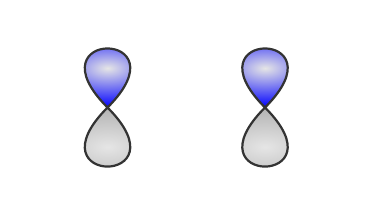
\begin{tikzpicture}
\orbital[pos={(0,0)}]{pz}
\orbital[pos={(2,0)}]{pz}
\end{tikzpicture}

\medskip Since one is + and the other is -, the overall reflection is -. 
}
\end{frame}

\begin{frame}
\frametitle{1\(^{st}\) and 2\(^{nd}\) row diatomics}
MOs have either \(\sigma\) or \(\pi\) aymmetry. \(\pi\)-symmetry involves a nodal plane.\newline
Allowed values
\[ -L \leqslant M_L \leqslant L \ ,\ -S \leqslant M_S \leqslant S\]
\medskip
\[ ^{2S+1}\Lambda\ ,\ where\  \Lambda = |M_L|\]
\bigskip\bigskip
\centering\fbox{\begin{tabular}{c c c c c}
\(\Lambda\) & 0 & 1 & 2 & 3\\
Symbol & \(\Sigma\) & \(\Pi\) & \(\Delta\) & \(\Phi\)\\
\end{tabular}}
\end{frame}

\begin{frame}
\frametitle{Term symbol H\(_2\) ground state}
Homonuclear datomics: \emph{g or u} (inversion center)\newline\bigskip
Heteronuclear diatomics: no inversion center\newline\bigskip
\textbf{\(H_2\):}\newline 2 electrons, both \(m_\ell=0 \implies \Lambda = 0\)\newline
\enspace Pauli: \(M_s = +\frac{1}{2} -\frac{1}{2} = 0 \implies S=0\)\newline\par
\quad it has g symmetry: \(^1\Sigma_g\) ground state \newline
\end{frame}

\begin{frame}
\frametitle{H\(_2\) 1\(^{st}\) and 2\(^{nd}\) excited states}
Configuration: \enspace (\(1\sigma_g)(1\sigma_u\)) : \quad \(e^-\) in separate MOs
\(m_l=0 \ for \ both \implies \Lambda = 0 \implies \Sigma\)-terms\newline
\(m_s = -1,0,0,1 \implies S=1 \ and \ S=0\newline
\implies\) Two excited states:
\(u \times g = u\) : both are u functions\newline
\[ Terms\ are\ ^3\Sigma_u \ and \ ^1\Sigma_u\]
Hund's rule: The triplet state is lower in energy\newline\begin{block}{nodal plane symmetry}
For \(\Sigma\) terms only: + or \(-\) symmetry\newline
Does the antisymmetrized molecular wavefunction change sign (-) or not (+) in a reflection through any plane containing the molecular axis?\end{block}
\end{frame}

\begin{frame}
\frametitle{Symmetry: + or - ?}
\begin{block}{quick rules: for the ground states}
If all MOs are filled: \textcolor{red}{+}

\medskip If all partially filled MOs have \(\sigma\) symmetry: \textcolor{red}{+}

\medskip For partially filled MOs of \(\pi\) symmetry (e.g. \(B_2\) and \(O_2\)), if \(\Sigma\)~terms arise:

\medskip \quad the triplet state is \textcolor{red}{\(-\)} and 

\medskip \quad the singlet state is \textcolor{red}{+}
\end{block}
\end{frame}

\begin{frame}
\frametitle{O\(_2\) molecular terms}
\only<1>{
Only the last two electrons in the configuration contribute to non-zero net values of \(M_L\) and \(M_S\):\newline
\( (1\sigma_g)^2(1\sigma_u^*)^2(2\sigma_g)^2(2\sigma_u^*)^2(3\sigma_g)^2(1\pi_u)^2(1\pi_u)^2\textcolor{red}{(1\pi_g*)^1(1\pi_g^*)^1}\)
}

\only<2>{
Neglecting Spin-Orbit coupling (more of that later):\newline
The total energy is independent of \(M_S\) and \(M_L\)\newline

There are 2L+1 possible values of \(M_L\) and 2S+1 possible values of \(M_S\)\\
So a term includes (2L+1)(2S+1) quantum states\\
 \bigskip
  (2S+1) is called the \emph{multiplicity}

\medskip Group of quantum states with same value of L and S but different values of \(M_L\) and \(M_S\) are degenerate in energy: This is called a \textit{Term}: \(^{2S+1}L\), where L = 0,1,2,3,... which are named S, P, D, F, G, ...
}

\only<3>{
The possible ways of combining the orbital and spin angular momenta of the last two electrons consistent with the Pauli principle are given in the table. The \(\Lambda\) values are determined as for atomic terms. M\(_L \leqslant L\)\newline\bigskip
\begin{tabular}{|c|c|p{1.5cm}|c|c|p{1.5cm}|c|}\hline
\(m_{l1}\) & \(m_{l2}\) & \(M_L = m_{l1} + m_{l2}\) & \(m_{s1}\) & \(m_{s2}\) & \(M_S = m_{s1} + m_{s2}\) & Term\\\hline
1 & 1 & 2 & +1/2 & -1/2 & 0 & \(^1\Delta\)\\
-1 & -1 & -2 & +1/2 & -1/2 & 0 & \(^1\Delta\)\\\hline
1 & -1 & 0 & +1/2 & +1/2 & 1 & \(^3\Sigma\)\\
1 & -1 & 0 & -1/2 & -1/2 & -1 & \(^3\Sigma\)\\\hline
1 & -1 & 0 & +1/2 & -1/2 & 0 & \(^1\Sigma, \ ^3\Sigma\)\\
1& -1 & 0 & -1/2 & +1/2 & 0 & \(^1\Sigma, \ ^3\Sigma\)\\\hline
\end{tabular}
}

\only<4>{
But what are the symmetries for \(O_2\)?

\medskip The two electrons in the \(\pi^*\) orbitals are both \textit{g}, so \(g + g = g\) and the parity label is g, so the term symbol is \(^1\Delta _g\). We do not assign reflection labels to non \(\Sigma\) states.

\medskip The \(\Sigma\) term has three possible spin configurations, so it is \(^3\Sigma\). Both orbitals are \textit{g}, so it is also a \textit{g}. One of the orbitals will be + and the other will be -. It is a \(^3\Sigma_g^+\)
}
\end{frame}

\includepdf[pages={2,3}, pagecommand={},frame=true,scale=0.8]{../../2018/Lectures/symmetry.pdf}

\subsection{Term symbols for diatomics and linear molecules}

\begin{frame}[<+->]
\frametitle{Electronic state and configuration for molecules}
\begin{itemize}
\item Primary quantum number, \emph{n}
\item Angular momentum quantum number, \emph{\(\Lambda\)}
\item spin quantum number, \emph{S}
\item the quantum number \(\Sigma\) (S, S-1, ... , -S)
\item the projection of the total angular momentum quantum number onto the molecular symmetry axis \(\Omega\):
\[\Omega = \Lambda + \Sigma\]
\item Term symbol \[^{2S+1}\Lambda^{(+/-)}_{\Omega,(g/u)}\]
\end{itemize}
\end{frame}

\subsection{Mulliken's labelling convention}

\begin{frame}
\frametitle{Energy order}
\only<1>{
If the ground state is singlet (or triplet), the excited states are singlets or triplets.

\smallskip If the ground state is a doublet (or quartet), the excited states are doublet or quartet.

\medskip Nomenclature:\newline
The \textit{ground state} is always X\newline
Excited states of the same spin are A, B, C, ...\newline
Excited states of different spin are a, b, c, ...\newline
Excited states are labelled in order of increasing energy

\medskip \textcolor{red}{E.g. O\(_2\): Ground state is \(X^3\Sigma^-_g\)}
}

\only<2>{
\begin{columns}[onlytextwidth]
\begin{column}{2in}
\includegraphics[width=1.5in]{../../graphics/oxygenenergy}
\end{column}
\begin{column}{4in}
\includegraphics[width=2.5in]{../../graphics/oxygenbands}
\end{column}
\end{columns}
}
\end{frame}

\section{Electronic selection rules}

\begin{frame}{What are selection rules?}
Selection rules describe the rules for which electronic transistions are \emph{allowed}. 
\end{frame}

\subsection{Selection rules for Atoms}

We say that the change in energy resulting from electronic transitions between states give rise to photon of energy \(\Delta E\). The frequency \(\nu\) is governed by the \textit{Bohr frequency condition:} \(h\nu = \Delta E\).

But this doesn't take into account angular momentum, so it is not the whole story. Photons possess angular momentum, just like electrons do. So the overall angular momentum has to be preserved in a transition as well. Therefore the electronic angular momentum must change by an amount that compensates for what is carried away by the spinning photon.

So an electron in a d-orbital (\(\ell = 2\)) cannot drop down into an s-orbital (\(\ell=0\)) with an emission of a photon because the emitted photon cannot carry away enough angular momentum. But a d-electron \textit{can} drop down to a p-orbital because \(\ell\) changes by 1 and the balance of the angular momentum can be carried away by the photon.

So some transitions are \textit{allowed} and others are \textit{forbidden}

\begin{frame}
\frametitle{Selection Rules for Atoms}
\only<1>{
As a reminder, the atomic term symbols are described by the following:
\begin{itemize}
\item The primary quantum number n
\item the angular momentum quantum number L
\item the spin quantum number S
\item the \textbf{total} angular momentum quantum number J
\end{itemize}

The final result is a term symbol of the form: \quad \(^{2S+1}L_J\)
}

\only<2>{
\medskip The selection rules are a set of rules that determine what changes in these numbers are allowed:
\begin{enumerate}
\item \(\Delta S = 0\)
\item \(\Delta L = 0,\pm 1\), but the L = 0 \(\leftrightarrow\) L = 0 transition is forbidden
\item \(\Delta J = 0, \pm 1\), but the J = 0 \(\leftrightarrow\) J = 0 transition is forbidden
\item \(\Psi_{initial}\) and \(\Psi_{final}\) must change in parity. \(\sum \ell_i\) odd or even. Only even \(\leftrightarrow\) transitions are allowed
\end{enumerate} 

Electronic spectra show the energies of the different transitions. Any transition, or peak, in a spectrum is associated with a change between two states described by different term symbols.
}

\only<3>{
\begin{enumerate}
\item \(\Delta S= 0\)
\item \(\Delta L = 0, \ \pm 1\), but \(L = 0 \leftrightarrow L=0\) transition forbidden
\item \(\Delta J = =0, \ \pm 1\), but \(J=0 \leftrightarrow J=0\) transition forbidden
\item \(\Psi_{initial}\) and \(\Psi_{final}\) must change in \emph{parity}. \(\sum \ell_i\) odd or even. only even \(\leftrightarrow\) odd transitions allowed.
\end{enumerate}
}
\end{frame}

\subsection{Selection rules for Molecules}

\begin{frame}
\frametitle{Selection rules for molecules}
\begin{enumerate}
\item \(\Delta S = 0 \ \Delta\Sigma = 0\)
\item \(\Delta\Lambda = 0, \pm1\)
\item Symmetry, g \(\leftrightarrow\) u allowed for homonuclear molecules\\
	+ \(\leftrightarrow\) + and \(- \leftrightarrow -\) allowed for heteronuclear molecules
\end{enumerate}
\bigskip
\begin{description}
\item[\(g \leftrightarrow u \)] applies to inversion through an inversion center in the molecule\newline
\item[\(+,\ -\)] applies to symmetry of molecular wavefunction reflecting against its symmetry axis
\end{description}
\end{frame}

%\section{Electronic Spectroscopy of Atoms}
%
%\section{Electronic Spectroscopy of Diatomic Molecules}
%
%In the following, we restrict our attention to diatomic molecules, similar to those that we
%have studied in rotational and vibrational spectroscopy.

\includegraphics[angle=90,origin=c,scale=0.7]{../../literature/MOs}



%\section{Additional Notes and examples}
%\includepdf[pages=-, pagecommand={},frame=true,scale=0.8]{../../2018/Lectures/CM3016_Lecture_handout_4}

\end{document}